\documentclass[preprint,12pt]{elsarticle}
\biboptions{sort&compress}
\usepackage{amsmath}
\usepackage{amsfonts}
\usepackage{amssymb}
\usepackage{bm}
\usepackage{graphicx}
\usepackage{hyperref}
\usepackage{tabls}
\usepackage{multirow}
\usepackage{cleveref}
\usepackage{verbatim}

\usepackage{pgfplots}
\usetikzlibrary{plotmarks}
\usepackage{tikz}
\usetikzlibrary{shapes,arrows}
\newcommand*{\h}{\hspace{5pt}}% for indentation
\newcommand*{\hh}{\h\h}% double indentation

\usepackage{framed} % Framing content
\usepackage{multicol} % Multiple columns environment
\usepackage{nomencl} % Nomenclature package
\RequirePackage{ifthen}
\renewcommand{\nomgroup}[1]{%
\ifthenelse{\equal{#1}{P}}{\item[\textbf{Superscripts}]}{
\ifthenelse{\equal{#1}{G}}{\item[\textbf{Greek Symbols}]}{
\ifthenelse{\equal{#1}{S}}{\item[\textbf{Subscripts}]}{}}}}

\newcommand{\nomunit}[1]{%
\renewcommand{\nomentryend}{\hspace*{\fill}#1}}

%\usepackage{breqn}

%\special{papersize=8.5in,11in}

\journal{International Journal of Heat and Mass Transfer}


\pdfinfo{%
  /Title    (Solution of an Inverse Convection Problem by a Predictor-Corrector Approach)
  /Author   (Yogesh Jaluria)
    /Author   (Joseph R VanderVeer)
  /Creator  (Joseph R VanderVeer)
  /Subject  (Inverse Convection Problems)
}

\begin{document}

\begin{frontmatter}
\title{Solution of an Inverse Convection Problem by a Predictor-Corrector Approach}

\author{Joseph R VanderVeer}
\author{Yogesh Jaluria\corref{cor}}
\ead{jaluria@soemail.rutgers.edu}

\address{Department of Mechanical and Aerospace Engineering: Rutgers University, 98 Brett Rd, Piscataway NJ, 08854}
\cortext[cor]{Corresponding Author}



\begin{abstract}
A predictor - corrector method for solving inverse convection problems has been developed and tested against both numerical and experimental data.  The method was applied to the simple convection problem of a two-dimensional plume in a crossflow.  Crossflow velocities up to $1.0\, m/s$.  The plume was generated by electrically heating a copper plate to a temperature up to $425\, K$.  The method attempts to predict both the source strength, and the source location, with a self imposed requirement on sampling and simulation data points.  The samples and simulations required are found to be 5 and 2 respectively.  Tests based on simulation alone indicate the methodology has a source strength prediction error of less than $1\%$ , and less than $6\%$ for source location.  Experimental tests bring the overall error upto $5\%$ for source strength and $10\%$ for source location.  This study indicates the potential of the methodology and demonstrates some of its limitations.  The approach can be extended to applied areas such as environmental flows, room fires, and thermal management systems.

\end{abstract}
\begin{keyword}
Inverse Problems \sep Computational Heat Transfer \sep Convection
\end{keyword}
\end{frontmatter}

\crefname{equation}{equation}{equations}
\crefname{figure}{figure}{figures}
\crefname{table}{table}{tables}

\newlength\figureheight 
\newlength\figurewidth 
	
	
	
	
\makenomenclature
\setlength{\nomitemsep}{-\parskip} % Baseline skip between items
\renewcommand*\nompreamble{\begin{multicols}{2}}
\renewcommand*\nompostamble{\end{multicols}}

\nomenclature[G]{$\rho$}{density}
\nomenclature[A]{$t$}{time}
\nomenclature[A]{$x,y$}{coordinates}
\nomenclature[A]{$u,v$}{velocity components}
\nomenclature[A]{$U$}{free stream velocity}
\nomenclature[A]{$P$}{pressure}
\nomenclature[A]{$E$}{thermal energy}
\nomenclature[A]{$T$}{temperature}
\nomenclature[G]{$\mu_{t}$}{eddy viscosity}
\nomenclature[A]{$P_{rt}$}{turbulent Prandtl number}
\nomenclature[A]{$k$}{turbulence kinetic energy}
\nomenclature[G]{$\epsilon$}{turbulence dissipation rate}
\nomenclature[A]{$C_1,C_2,C_{1\epsilon},C_{\mu},\sigma_k,\sigma_{\epsilon}$}{$k-\epsilon$ model coefficients}
\nomenclature[A]{$l$}{turbulence length scale}
\nomenclature[A]{$I$}{turbulence intensity}
\nomenclature[A]{$X,Y$}{normalized coordinates}
\nomenclature[A]{$n$}{number of sample locations}
\nomenclature[A]{$d$}{number of simulations}
\nomenclature[G]{$\phi$}{normalized temperature $\phi = \frac{T-T_{\infty}}{T_S-T_{\infty}}$}
\nomenclature[S]{$i, j,k$}{index}
\nomenclature[S]{$A,B$}{data set A,B}
\nomenclature[S]{$P$}{predicted}
\nomenclature[S]{$mod$}{modified}
\nomenclature[S]{$\infty$}{free stream}
\nomenclature[P]{$\ast$}{predictor stage, alternative heat flux eqn.}
\nomenclature[S]{$S$}{source}
\nomenclature[G]{$\lambda$}{thermal conductivity}
\nomenclature[A]{$F$}{minimization function}
\nomenclature[A]{$M_W$}{molecular weight}
\nomenclature[A]{$b,m$}{model parameters}
\nomenclature[G]{$\mu$}{dynamic viscosity}
\nomenclature[P]{$'$}{instantaneous}
\nomenclature[P]{$-$}{ensemble averaged}
\nomenclature[A]{ }{ }

\begin{table*}[!t]
  \begin{framed}
    \printnomenclature
  \end{framed}
\end{table*}

\section{Introduction}

Inverse heat transfer problems are often of greater interest to engineers than the associated forward problems.  An example of this consideration is the temperature distribution on the wall of an optical fiber drawing furnace.  The temperature at the center of the furnace is relatively easy to measure using an instrumented graphite rod.  The temperature at the walls of the furnace is very difficult to measure due to the cylindrical shape of the furnace, inaccessibility, and high temperatures.  \citet{issa} developed a regularization technique to use the center line temperature to predict the furnace wall temperature.  Thus an inverse problem was solved and optimization was used to make the final result essentially unique.


Many methods are available to solve inverse problems.  Several books \cite{tikhonov, tikhonov2, ozisik, orlande} and articles \cite{invconduction,invradiation,jones,daun,mossi,erturk} have been published on the subject.  However few articles cover the inverse convection problems, and those that do often cover it as an aside to radiative or conduction problems.  Of the few articles available, often a simple yet effective method is used to solve the inverse convection problem.  That method is to iterate the simulation until it matches the known data, often requiring many iterations.  This would be time consuming in large and complicated domains.  One such example is the paper by \citet{liu}, in which they use inverse convection methods to determine thermal profiles in a slot vented enclosure.  They use this iterative approach requiring 20 to 30 iterations to achieve less than $1\%$ error.  

\citet{knight} used an iterative experimental-numerical data driven approach, coupled with a response surface, to predict the temperature and velocity of a jet in a crosswind.  This method helps in predicting which data points need to be sampled in between iterations.  They found that the methodology was able to predict jet velocity within experimental uncertainty and source temperature within $9\%$.  However, the second stage of their approach over-predicted source temperature by as much as $23\%$ \cite{knight,rossmann}.

The present study is a continuation of the work initiated by \citet{knight} and \citet{rossmann}.  Preliminary work was covered in \cite{cht12}, with the sole purpose of being able to predict the source location as well as source strength.  The added complexity of the unknown source location warranted an overall simplification of the problem from a jet in a crosswind to a plume in a crosswind.  The overall goal is to predict, within acceptable error, both the location and source strength of the plume.  For this methodology to be most useful, the number of sample points must be limited to a select few, and the number of simulations also must be kept small.

\section{Experimental System}
Most inverse solution methodologies require a fundamental understanding of the forward problem.  This particular method is no different.  As previously described, the forward problem is a plume of heated air in a crosswind.  A small region heated to a given temperature $T_S$ is subjected to a flow of velocity $U_\infty$, which is perpendicular to the direction of the vertical flow induced by thermal buoyancy.

The wind tunnel test section dimensions are $54.5\times 305\times 254\, mm$, and can produce velocities in the range of $0-5.0\, m/s$.  \Cref{fig:diagram} is a schematic of the experimental wind tunnel including the computational domain.  All dimensions are in millimeters and the depth into the page is $305\, mm$.  The heated section uses a resistance type electric heater to heat a copper block, encouraging a uniform heated surface, which is $25.4\, mm$ wide.  The maximum temperature of the heated section is limited to a maximum of $450\, K$ due to material limitations of the wind tunnel.  This creates a limitation to the maximum free stream velocity within the tunnel as the maximum heat input gets overwhelmed by the free stream above $1.0\, m/s$.  That is to say the thermal plume is difficult to detect using the methods described here.  The temperatures are measured using a K-type thermocouple mounted on a two-dimensional stage for motion within the plane of the figure.  The X-direction is in the direction of the free stream, with zero at the upstream edge of the heated block.  The Y-direction is in the direction of the plume, with zero at the surface of the heater.  

A Pitot-static tube is used to determine the free stream velocity.  The tube is attached to a NIST traceable differential pressure sensor from Omega (PX655-0.1DI), which has a full scale reading of $0.1$ inches of water.  The pressure sensor has an error of $0.05\%$ of full scale reading.  This results in a maximum of $3\%$ error of the calculated velocity, which is at most $0.018\, m/s$ for the applicable velocities.

The temperature is measured using a K-type thermocouple probe mounted on an X-Y traversing stage, and recorded using a National Instruments data acquisition board.  Samples over several days yield a maximum difference of $7\%$ outside the plume, and a maximum of $2\%$ within the plume, indicating good repeatability.


\begin{figure*}[!tbp]
\begin{center}
\includegraphics[scale=.30]{WindTunnel.jpg}
\caption{Schematics of the wind tunnel and the computational domain \cite{cht12}}
\label{fig:diagram}
\end{center}
\end{figure*}

\section{Numerical Simulations}

The numerical simulations were carried out using the software package Ansys Fluent version 13\cite{fluentsoftware}.  The Navier-Stokes equations were solved using a three dimensional, steady state, realizable $k-\epsilon$ model with enhanced wall effects.  The three-dimensional model is employed due to a limitation of Fluent, solid-solid conduction is not modeled at all in two-dimensional conjugate heat transfer problems, and the desire to ensure two dimensionality of the flow.  The flow is relatively slow and often in the transient transitional turbulence regime with oscillating characteristics.  The Reynolds number is of order 2000.  The Richardson number was calculated and found to be of the order 5 and thus buoyancy introduces a non-negligible amount of turbulence into the flow.



The governing equations are given as:

\begin{equation}
\centering
u_i = \overline{u_i} + u^{'}_{i}
\label{eq:veldecomp}
\end{equation}

\begin{equation}
\frac{\partial \rho }{\partial t } + \frac{\partial }{\partial x_i} \left( \rho u_i \right) = 0 
\label{eq:mass}
\end{equation}

\begin{equation}
\centering
\begin{split}
\frac{\partial }{\partial t} \left( \rho u_i \right) &+ \frac{\partial }{\partial x_j } \left( \rho u_i u_j \right) = \\
 &\frac{\partial P}{\partial x_i } + \frac{\partial }{\partial x_j } \left[ \mu \left( 2 S_{ij} - \frac{2}{3} \delta_{ij} \frac{\partial u_k }{\partial x_k } \right) - \rho \overline{u^{'}_{i} u^{'}_{j}} \right] 
\label{eq:momentum}
\end{split}
\end{equation}

\begin{equation}
\centering
\begin{split}
\frac{\partial }{\partial t } \left( \rho E \right) &+ \frac{\partial }{\partial x_i} \left[ u_i \left( \rho E + P \right) \right] = \\
 &\frac{\partial }{\partial x_i } \left[ \left( \lambda + \frac{C_p \mu_t }{P_{rt}} \right) \frac{\partial T}{\partial x_i} \right] 
\label{eq:energy}
\end{split}
\end{equation}

\begin{equation}
\centering
\begin{split}
\frac{\partial }{\partial t} \left(\rho k \right) &+ \frac{\partial }{\partial x_j} \left( \rho k u_j \right) = \\
&\frac{\partial }{\partial x_j} \left[ \left( \mu + \frac{\mu_t}{\sigma_k} \right) \frac{\partial k}{\partial x_j} \right] + \frac{\partial u_j}{\partial x_i} \left( -\rho \overline{u^{'}_{i} u^{'}_{j}} \right) \\
&- g_i \frac{\mu_t}{\rho P_{rt}} \frac{\partial \rho }{\partial x_i} + \rho \epsilon
\label{eq:k}
\end{split}
\end{equation}

\begin{equation}
\centering
\begin{split}
 \frac{\partial }{\partial t} \left(\rho \epsilon \right) &+ \frac{\partial }{\partial x_j} \left( \rho \epsilon u_j \right) = \\
 &\frac{\partial }{\partial x_j } \left[ \left( \mu + \frac{\mu_t }{\sigma_\epsilon } \right) \frac{\partial \epsilon }{\partial x_j } \right] + \rho C_1 S \epsilon - \rho C_2 \frac{\epsilon^2 }{k+\sqrt{\nu \epsilon}} \\
 &- C_{1 \epsilon} \frac{\epsilon}{k} C_{3\epsilon} g_i \frac{\mu_t}{\rho P_{rt}} \frac{\partial \rho}{\partial x_i}
\label{eq:e}
\end{split}
\end{equation}

\begin{equation}
\centering
- \rho \overline{u^{'}_{i} u^{'}_{j}} = 2\mu_t S_{ij} - \frac{2}{3} \delta_{ij} \left( \rho k + \mu_t \frac{\partial u_k}{\partial x_k} \right)
\label{eq:reynoldsstress}
\end{equation}

\Cref{eq:veldecomp} gives the averaging employed.  \Cref{eq:mass,eq:momentum,eq:energy} are the equations for conservation of mass, momentum, and energy, respectively.  \Cref{eq:k,eq:e} are the turbulent kinetic energy and dissipation equations.  \Cref{eq:reynoldsstress} is the Reynolds stress equation.  $\delta_{ij}$ is the kronecker delta.

The constants for the turbulence model are \cite{realizable} : 
\begin{equation}
\label{eq:constants}
C_{1\epsilon} = 1.44 , C_2 = 1.9 , \sigma_k = 1.0 , \sigma_\epsilon = 1.2 , P_{rt} = 0.85 
\end{equation}
%
The coefficients of the model are \cite{fluent}:
\begin{equation}
C_1 = max\left[0.43,\frac{Sk/\epsilon}{Sk/\epsilon +5} \right] , S = \sqrt{2S_{ij}S_{ji}} , C_{3\epsilon} = tanh\left(\frac{u_g}{u_p}\right)
\end{equation}
%
Where the $u_g$ is the velocity component parallel to gravity, and $u_p$ is the velocity perpendicular to gravity.  

The realizable $k-\epsilon$ model varies from the traditional model by using a non-constant coefficient $C_\mu$ of the eddy viscosity equation $\mu_t$.  Which is defined as follows \cite{fluent,realizable}
%
\begin{subequations}
\begin{align}
\mu_t &= \frac{\rho C_{\mu} k^2}{\epsilon} \\
C_{\mu} &= \frac{1}{A_0 + \frac{A_1 k U^*}{\epsilon}} \\
U^* &\equiv \sqrt{S_{ij} S_{ji} + \Omega_{ij} \Omega_{ji}} \\
A_0 &= 4.04 \\
A_1 &= \sqrt{6} cos \left[\frac{1}{3} cos^{-1}\left(\sqrt{6} \frac{S_{ij}S_{jk}S_{ki}}{\left(S_{ij} S_{ji} \right)^{\frac{3}{2}}} \right) \right] \\
S_{ij} &= \frac{1}{2} \left( \frac{\partial u_i}{\partial x_j} + \frac{\partial u_j}{\partial x_i} \right) \\
\Omega_{ij} &= \frac{1}{2} \left( \frac{\partial u_i}{\partial x_j} - \frac{\partial u_j}{\partial x_i} \right)
\end{align}
\end{subequations}
%
$S_{ij}$ and $\Omega_{ij}$ are the strain rate tensor and the angular velocity tensor respectively.  The fluid is modeled as an ideal gas at atmospheric pressure.  Specific heat at constant pressure is taken as constant at $C_P=1006.43\, J/(kg-K)$.  The dynamic viscosity and thermal conductivity are both modeled using the Chapman-Enscog equations, listed below, with constant Lennard-Jones parameters of $\sigma = 3.711\,\textup{\AA}$ and $\frac{\epsilon}{k_B} = 78.6\, K$.  Where $\Omega_{\mu}$ is the collision integral for viscosity, for more information see \citet{vincenti,fluent}.
\begin{subequations}
\begin{align}
\mu &= 2.67 \times 10^{-6} \frac{\sqrt{M_W T}}{\sigma^2 \Omega_{\mu} \left(\frac{T}{\epsilon/k_B} \right)} \\
\lambda &= \mu \left(\frac{5}{4} \frac{R}{M_W} +C_P \right)
\end{align}
\end{subequations}


The inflow boundary conditions are:
\begin{subequations}
\label{eq:inflow}
\begin{align}
u&=U_\infty , v=0 , T=T_\infty , P = P_\infty , l=4 mm , I=5\%\\
k&=\frac{3}{2}\left(U_\infty I\right)^2 \\
\epsilon &=C_{\mu}^{3/4} \frac{k^{3/2}}{l}
\end{align}
\end{subequations}
%
The boundary conditions imposed are as follows:  Since upper boundary is very far from the plume flow and should have negligible effect on the result, a symmetric boundary was used.  This would reduce the errors possibly introduced by the experimentally accurate no-slip condition.  The exit is a pressure outflow set to $P_{\infty}$.  The bottom boundary has seven zones as described in \cref{fig:diagram}, from left to right: acrylic, ceramic, heated copper, ceramic, unheated copper, ceramic, and acrylic.  All of the material properties are taken as constant.  The ceramic is a ceramic/aero-gel that has effective density, specific heat, and thermal conductivity of $2330\, kg/m^3$, $1138 \, J/(kg-K)$, and $0.1\, W/(m-K)$, respectively.  The density was calculated from the unaccounted mass of the mould used to cast the ceramic and the filled volume of said mould.  The specific heat is that of the ceramic obtained from the manufacturer, Coitronics.  The thermal conductivity was determined via approximation between the ceramic and the aero-gel wrapping.

The bottom is simulated with conjugate heat transfer, with an effective layer width of $25.4\, mm$ and an effective outer temperature of $T_{\infty}$.  The outer layer temperature for the heated copper region is taken as $T_S$ \cite{cht12}.

\subsection{Simulation Validation}

Grid independence is demonstrated with a comparison of the simulated temperature at a few locations, with varying element counts.  \Cref{tab:grid}, shows the results for the conditions tested.  The result is a variation of a fraction of a percent.  With the wide range of element count, and little change in the result, one must come to the conclusion that the result is independent of the grid.  The grid employed is an unstructured hexagonal mesh with emphasis located at the bottom surface of the wind tunnel and down stream of the plume.

\begin{table}[!h!t!b!p]
\begin{center}
\begin{tabular}{ c c c c c }
 Location (x,y) (mm) & 30,2 & 35,3 & 40,1 & 50,10 \\ \hline \hline
 Element Count & \\ \hline
 67399  & 360.3 & 338.5 & 352.9 & 295.6 \\ \hline
 94378  & 360.2 & 338.6 & 352.7 & 295.6 \\ \hline
 130292 & 360.2 & 338.5 & 352.7 & 295.6 \\ \hline
 153290 & 360.1 & 338.8 & 352.6 & 295.8 \\ \hline
\end{tabular}
\caption{Grid Independence Study \cite{cht12}}
\label{tab:grid}
\end{center}
\end{table}
%
The simulation and experimental conditions of the previous table and the following two graphs are shown in here, \cref{tab:VT}.

\begin{table}[!h!t!b!p]
\begin{center}
\begin{tabular}{ c c }
Parameter    & Value \\ \hline
$U_{\infty} \, (m/s)$ & $0.6\pm0.15$ \\
$T_{\infty} \, (K) $ & $294.5\pm2.0$ \\
$P_{\infty} \, (kPa) $ & $101.6\pm0.2$ \\
$T_{S} \, (K) $ & $433\pm2.0$ \\
\end{tabular}
\caption{Validation Test \cite{cht12}}
\label{tab:VT}
\end{center}
\end{table}

To validate the simulation, a comparison directly with the experimental results was performed.  Two slices of the compared data are shown in \cref{fig:simVSexpX40,fig:simVSexpX70}.  The data has been normalized via \cref{eq:normalize}, where L is the width of the heated region.  The trend in the numerical simulations tends to overshoot the experimental results, albeit the overshoot is minor.  The error within the region of interest where the bulk of the plume resides, is less than $2\%$, and often even less than $1\%$.  Having the numerical simulations match the experimental results so closely is key to allowing the following methodology to function as well as it does.

\begin{figure}[!htbp]
	\centering
  \setlength\figureheight{6cm} 
	\setlength\figurewidth{6cm}
	% This file was created by matlab2tikz v0.2.1.
% Copyright (c) 2008--2012, Nico Schlömer <nico.schloemer@gmail.com>
% All rights reserved.
% 
% The latest updates can be retrieved from
%   http://www.mathworks.com/matlabcentral/fileexchange/22022-matlab2tikz
% where you can also make suggestions and rate matlab2tikz.
% 
% 
% 
\begin{tikzpicture}

\begin{axis}[%
view={0}{90},
width=\figurewidth,
height=\figureheight,
scale only axis,
xmin=0, xmax=1,
xlabel={Normalized Temperature},
ymin=0, ymax=0.5,
ylabel={Normalized Distance Above Surface (Y-axis)},
legend style={nodes=right}]
\addplot [
color=black,
solid
]
coordinates{
 (0.460687772793034,0)(0.460441266447345,0.0025)(0.460194760101656,0.005)(0.459948253755968,0.0075)(0.459701747410279,0.01)(0.45945524106459,0.0125)(0.459310527716331,0.015)(0.459233521323468,0.0175)(0.459156514930604,0.02)(0.45907950853774,0.0225)(0.459002502144876,0.025)(0.458925495752013,0.0275)(0.458547683525903,0.03)(0.456771821897319,0.0325)(0.454995960268735,0.035)(0.453220098640151,0.0375)(0.451444237011567,0.04)(0.449668375382983,0.0425)(0.448046637658835,0.045)(0.446470856659523,0.0475)(0.44489507566021,0.05)(0.443319294660898,0.0525)(0.441743513661586,0.055)(0.440167732662273,0.0575)(0.43796911469207,0.06)(0.433904928730671,0.0625)(0.429840742769272,0.065)(0.425776556807873,0.0675)(0.421712370846474,0.07)(0.417648184885075,0.0725)(0.413735892771499,0.075)(0.409859937159638,0.0775)(0.405983981547776,0.08)(0.402108025935915,0.0825)(0.398232070324054,0.085)(0.394356114712193,0.0875)(0.389872431869952,0.09)(0.384125276062302,0.0925)(0.37837812025465,0.095)(0.372630964447,0.0975)(0.366883808639349,0.1)(0.361136652831698,0.1025)(0.355472267409053,0.105)(0.349977903706415,0.1075)(0.344483540003777,0.11)(0.33898917630114,0.1125)(0.333494812598502,0.115)(0.328000448895864,0.1175)(0.322506085193226,0.12)(0.316847412008303,0.1225)(0.310545176628765,0.125)(0.304242941249226,0.1275)(0.297940705869688,0.13)(0.291638470490149,0.1325)(0.28533623511061,0.135)(0.279096863273417,0.1375)(0.273059822360866,0.14)(0.267022781448315,0.1425)(0.260985740535763,0.145)(0.254948699623213,0.1475)(0.248911658710662,0.15)(0.242874617798111,0.1525)(0.236898215959193,0.155)(0.231739178185081,0.1575)(0.226580140410968,0.16)(0.221421102636856,0.1625)(0.216262064862744,0.165)(0.211103027088631,0.1675)(0.205943989314519,0.17)(0.200784951540407,0.1725)(0.195625913766294,0.175)(0.190503498576307,0.1775)(0.185414296145811,0.18)(0.180325093715315,0.1825)(0.175235891284818,0.185)(0.170146688854322,0.1875)(0.165057486423825,0.19)(0.159968283993329,0.1925)(0.154879081562833,0.195)(0.150967541967099,0.1975)(0.147489649225661,0.2)(0.144011756484224,0.2025)(0.140533863742787,0.205)(0.13705597100135,0.2075)(0.133578078259912,0.21)(0.130100185518476,0.2125)(0.126622292777038,0.215)(0.123144400035601,0.2175)(0.119666507294164,0.22)(0.116190390739182,0.2225)(0.112714422216661,0.225)(0.109238453694139,0.2275)(0.105762485171618,0.23)(0.102286516649096,0.2325)(0.0988105481265752,0.235)(0.095334579604054,0.2375)(0.0918586110815332,0.24)(0.0890888580921317,0.2425)(0.0870101978666839,0.245)(0.0849315376412357,0.2475)(0.0828528774157884,0.25)(0.0807742171903407,0.2525)(0.0786955569648929,0.255)(0.0766168967394452,0.2575)(0.0745382365139974,0.26)(0.0724595762885497,0.2625)(0.0703809160631019,0.265)(0.0683022558376537,0.2675)(0.0662288743957264,0.27)(0.0641558397608521,0.2725)(0.0620828051259778,0.275)(0.0600097704911034,0.2775)(0.0579367358562291,0.28)(0.0558637012213548,0.2825)(0.0537906665864804,0.285)(0.0517176319516061,0.2875)(0.0496445973167322,0.29)(0.048368435163902,0.2925)(0.0471843657209687,0.295)(0.0460002962780358,0.2975)(0.0448162268351025,0.3)(0.0436321573921696,0.3025)(0.0424480879492363,0.305)(0.0412640185063029,0.3075)(0.04007994906337,0.31)(0.0388958796204367,0.3125)(0.0377118101775039,0.315)(0.0365599260674086,0.3175)(0.0354420760624008,0.32)(0.0343242260573926,0.3225)(0.0332063760523844,0.325)(0.0320885260473762,0.3275)(0.0309706760423684,0.33)(0.0298528260373606,0.3325)(0.0287349760323519,0.335)(0.0276171260273441,0.3375)(0.0264992760223359,0.34)(0.0257987850580805,0.3425)(0.0252115206699682,0.345)(0.0246242562818559,0.3475)(0.0240369918937431,0.35)(0.0234497275056304,0.3525)(0.0228624631175181,0.355)(0.0222751987294054,0.3575)(0.0216879343412926,0.36)(0.0211006699531803,0.3625)(0.0205134055650676,0.365)(0.0199261411769548,0.3675)(0.0193360135231009,0.37)(0.0187253456801132,0.3725)(0.0181146778371251,0.375)(0.0175040099941374,0.3775)(0.0168933421511493,0.38)(0.0162826743081616,0.3825)(0.0156720064651734,0.385)(0.0150613386221853,0.3875)(0.0144506707791972,0.39)(0.0138400029362095,0.3925)(0.013391007557779,0.395)(0.013094368485708,0.3975)(0.0127977294136365,0.4)(0.012501090341565,0.4025)(0.012204451269494,0.405)(0.0119078121974229,0.4075)(0.0116111731253515,0.41)(0.0113145340532804,0.4125)(0.0110178949812094,0.415)(0.0107212559091379,0.4175)(0.0104246168370664,0.42)(0.0101213801830347,0.4225)(0.00981553476211075,0.425)(0.00950968934118634,0.4275)(0.00920384392026194,0.43)(0.00889799849933797,0.4325)(0.00859215307841399,0.435)(0.00828630765748916,0.4375)(0.00798046223656518,0.44)(0.00767461681564078,0.4425)(0.00736877139471637,0.445)(0.0070629259737924,0.4475)(0.00675708055286799,0.45)(0.00654826341186887,0.4525)(0.0064058551161953,0.455)(0.00626344682052217,0.4575)(0.00612103852484817,0.46)(0.00597863022917503,0.4625)(0.00583622193350147,0.465)(0.00569381363782747,0.4675)(0.00555140534215391,0.47)(0.00540899704648077,0.4725)(0.00526658875080677,0.475)(0.00512418045513321,0.4775)(0.0049814919572651,0.48)(0.00483199049002127,0.4825)(0.00468248902277701,0.485)(0.00453298755553318,0.4875)(0.00438348608828891,0.49)(0.00423398462104508,0.4925)(0.00408448315380082,0.495)(0.00393498168655655,0.4975)(0.00378548021931272,0.5) 
};

\addlegendentry{Simulation};

\addplot [
color=black,
only marks,
mark=o,
mark options={solid}
]
coordinates{
 (0.447132523559074,0)(0.433258602957899,0.0277777777777778)(0.419384682356724,0.0555555555555556)(0.405510761755549,0.0833333333333333)(0.361538143115063,0.111111111111111)(0.281758452669192,0.138888888888889)(0.201978762223319,0.166666666666667)(0.122199071777447,0.194444444444444)(0.0895953450278784,0.222222222222222)(0.0614652010426147,0.25)(0.033335057057351,0.277777777777778)(0.0144482595157174,0.305555555555556)(0.0112948176228153,0.333333333333333)(0.00814137572991319,0.361111111111111)(0.0049879338370111,0.388888888888889)(0.00422342796473073,0.416666666666667)(0.00395946106819939,0.444444444444444)(0.00369549417166805,0.472222222222222)(0.00356524389021579,0.5) 
};

\addlegendentry{Experiment};

\end{axis}
\end{tikzpicture}

	\caption{Validation of the simulation: Experiment versus simulation at $X=1.6$}
	\label{fig:simVSexpX40}
\end{figure}
\begin{figure}[!htbp]
	\centering
	\setlength\figureheight{6cm} 
	\setlength\figurewidth{6cm}
	% This file was created by matlab2tikz v0.2.1.
% Copyright (c) 2008--2012, Nico Schlömer <nico.schloemer@gmail.com>
% All rights reserved.
% 
% The latest updates can be retrieved from
%   http://www.mathworks.com/matlabcentral/fileexchange/22022-matlab2tikz
% where you can also make suggestions and rate matlab2tikz.
% 
% 
% 
\begin{tikzpicture}

\begin{axis}[%
view={0}{90},
width=\figurewidth,
height=\figureheight,
scale only axis,
xmin=0, xmax=1,
xlabel={Normalized Temperature},
ymin=0, ymax=0.5,
ylabel={Normalized Distance Above Surface (Y-axis)},
legend style={nodes=right}]
\addplot [
color=black,
solid
]
coordinates{
 (0.265849299570503,0)(0.265251395614334,0.0025)(0.264653491658166,0.005)(0.264055587701997,0.0075)(0.263432445714357,0.01)(0.262779964611485,0.0125)(0.262127483508614,0.015)(0.261475002405742,0.0175)(0.260822521302871,0.02)(0.260170040199998,0.0225)(0.259517559097127,0.025)(0.258865077994255,0.0275)(0.258190852944391,0.03)(0.257415568976311,0.0325)(0.256640285008232,0.035)(0.255865001040153,0.0375)(0.255089717072074,0.04)(0.254314433103994,0.0425)(0.253539149135915,0.045)(0.252763865167836,0.0475)(0.251988581199757,0.05)(0.251251348741898,0.0525)(0.250527256978487,0.055)(0.249803165215076,0.0575)(0.249038362563192,0.06)(0.247932698546852,0.0625)(0.246827034530512,0.065)(0.245721370514172,0.0675)(0.244610322382556,0.07)(0.243493278716514,0.0725)(0.242376235050473,0.075)(0.241259191384431,0.0775)(0.24014214771839,0.08)(0.239025104052348,0.0825)(0.237908060386307,0.085)(0.236791016720265,0.0875)(0.235673973054223,0.09)(0.234055794242493,0.0925)(0.232376976554963,0.095)(0.230698158867433,0.0975)(0.229019341179904,0.1)(0.227340523492374,0.1025)(0.225661705804843,0.105)(0.223982888117314,0.1075)(0.222304070429785,0.11)(0.220635476360137,0.1125)(0.219000492787613,0.115)(0.21736550921509,0.1175)(0.215730525642565,0.12)(0.213888021043504,0.1225)(0.211755544745416,0.125)(0.209623068447328,0.1275)(0.207490592149239,0.13)(0.205358115851151,0.1325)(0.203225639553062,0.135)(0.201093163254974,0.1375)(0.198960686956885,0.14)(0.196828210658797,0.1425)(0.194695734360708,0.145)(0.192546992939557,0.1475)(0.190347294859427,0.15)(0.188147596779297,0.1525)(0.185947898699166,0.155)(0.183735993273586,0.1575)(0.181336356453679,0.16)(0.178936719633772,0.1625)(0.176537082813865,0.165)(0.174137445993958,0.1675)(0.171774045076072,0.17)(0.169458519067967,0.1725)(0.167142993059861,0.175)(0.164827467051756,0.1775)(0.16251194104365,0.18)(0.160196415035545,0.1825)(0.15788088902744,0.185)(0.155565363019334,0.1875)(0.153249837011229,0.19)(0.150934311003124,0.1925)(0.148618784995018,0.195)(0.146329249319052,0.1975)(0.14416350619745,0.2)(0.141997763075849,0.2025)(0.139832019954248,0.205)(0.137666276832647,0.2075)(0.135501578164815,0.21)(0.133362969713688,0.2125)(0.13122436126256,0.215)(0.129085752811433,0.2175)(0.126947144360306,0.22)(0.124808535909178,0.2225)(0.122669927458051,0.225)(0.120531319006923,0.2275)(0.118392710555796,0.23)(0.116254102104669,0.2325)(0.114115493653542,0.235)(0.111976885202415,0.2375)(0.109838276751287,0.24)(0.107931364133336,0.2425)(0.106056815325731,0.245)(0.104182266518126,0.2475)(0.102307717710521,0.25)(0.100433168902916,0.2525)(0.0986089555175577,0.255)(0.0968083946469928,0.2575)(0.0950078337764275,0.26)(0.0932072729058627,0.2625)(0.0914067120352974,0.265)(0.0896061511647325,0.2675)(0.0878055902941672,0.27)(0.0860050294236024,0.2725)(0.0842044685530371,0.275)(0.0824039076824722,0.2775)(0.0806033468119065,0.28)(0.0788027859413416,0.2825)(0.0772431837162981,0.285)(0.0759462644707535,0.2875)(0.0746493452252089,0.29)(0.0733524259796638,0.2925)(0.0720555067341188,0.295)(0.0707585874885742,0.2975)(0.0694592149538944,0.3)(0.0681396758506598,0.3025)(0.0668201367474248,0.305)(0.0655005976441898,0.3075)(0.0641810585409547,0.31)(0.0628615194377201,0.3125)(0.0615419803344855,0.315)(0.0602224412312505,0.3175)(0.0589029021280159,0.32)(0.0575833630247809,0.3225)(0.0562638239215463,0.325)(0.0549442848183109,0.3275)(0.0536247457150767,0.33)(0.0523052066118417,0.3325)(0.0510951689871268,0.335)(0.0502100191704569,0.3375)(0.0493248693537874,0.34)(0.048439719537117,0.3425)(0.0475545697204471,0.345)(0.0466694199037772,0.3475)(0.0457842700871073,0.35)(0.0449005766346645,0.3525)(0.0440180859786933,0.355)(0.0431355953227213,0.3575)(0.0422531046667498,0.36)(0.0413706140107778,0.3625)(0.0404881233548062,0.365)(0.0396056326988342,0.3675)(0.0387231420428626,0.37)(0.0378406513868911,0.3725)(0.0369581607309191,0.375)(0.0360756700749479,0.3775)(0.0351931794189759,0.38)(0.0343106887630039,0.3825)(0.0334281981070323,0.385)(0.0325457074510603,0.3875)(0.0316817872167453,0.39)(0.0311200787164186,0.3925)(0.0305583702160932,0.395)(0.0299966617157669,0.3975)(0.0294349532154406,0.4)(0.0288732447151143,0.4025)(0.0283115362147881,0.405)(0.0277484994629068,0.4075)(0.0271766920575537,0.41)(0.0266048846522007,0.4125)(0.0260330772468477,0.415)(0.0254612698414946,0.4175)(0.0248894624361416,0.42)(0.0243176550307885,0.4225)(0.0237458476254359,0.425)(0.0231740402200829,0.4275)(0.0226022328147298,0.43)(0.0220304254093772,0.4325)(0.0214586180040238,0.435)(0.0208868105986712,0.4375)(0.0203150031933177,0.44)(0.0197431957879651,0.4425)(0.0191713883826125,0.445)(0.0186515454641441,0.4475)(0.0183108714921405,0.45)(0.0179701975201378,0.4525)(0.0176295235481338,0.455)(0.017288849576131,0.4575)(0.0169481756041279,0.46)(0.0166075016321247,0.4625)(0.0162668276601211,0.465)(0.0159261536881184,0.4675)(0.0155854797161152,0.47)(0.0152448057441121,0.4725)(0.0149041317721085,0.475)(0.0145634578001053,0.4775)(0.0142227838281022,0.48)(0.013882109856099,0.4825)(0.0135414358840959,0.485)(0.0132007619120927,0.4875)(0.0128660462961543,0.49)(0.0125333410630983,0.4925)(0.0122006358300419,0.495)(0.0118679305969855,0.4975)(0.0115352253639291,0.5) 
};

\addlegendentry{Simulation};

\addplot [
color=black,
only marks,
mark=o,
mark options={solid}
]
coordinates{
 (0.232031606014447,0)(0.233319199585032,0.0277777777777778)(0.234606793155618,0.0555555555555556)(0.235894386726203,0.0833333333333333)(0.224689825971879,0.111111111111111)(0.198623909210336,0.138888888888889)(0.172557992448792,0.166666666666667)(0.146492075687249,0.194444444444444)(0.116650327577323,0.222222222222222)(0.0864505264947051,0.25)(0.0562507254120876,0.277777777777778)(0.0337980169638536,0.305555555555556)(0.0245318491698902,0.333333333333333)(0.0152656813759258,0.361111111111111)(0.00599951358196233,0.388888888888889)(0.00350492018533018,0.416666666666667)(0.00242913285290084,0.444444444444444)(0.00135334552047106,0.472222222222222)(0.000563010863310962,0.5) 
};

\addlegendentry{Experiment};

\end{axis}
\end{tikzpicture}

	\caption{Validation of the simulation: Experiment versus simulation at $X=2.25$}
	\label{fig:simVSexpX70}
\end{figure}

\begin{subequations}
\label{eq:normalize}
\begin{align}
\phi &= \frac{T-T_{\infty}}{T_S-T_{\infty}} \\
X &= \frac{x}{L} \\
Y &= \frac{y}{L} 
\end{align}
\end{subequations}




\section{Methodology}
If we can neglect variations in density and buoyancy effects, the energy equation is decoupled from mass and momentum.  In neglecting variations in density and thermal buoyancy, the relation between the source temperature and the local static temperature becomes linear if thermal radiation is negligible, as shown in \cref{eq:linear,eq:m,eq:b}, where the subscripts $A$ and $B$ denote different simulations,  i.e. $T_{SA}$ is the source temperature of simulation A, and $T_A\left( x,y \right)$ is the local static temperature at $x,y$ for simulation A.

\begin{subequations}
\label{eq:linearset}
\begin{align}
T_S &= m\left( x,y \right) T\left( x,y \right) + b\left( x,y \right) \label{eq:linear} \\
m\left( x,y \right) &= \frac{T_{SA} - T_{SB}}{T_A \left( x,y \right) - T_B\left( x,y \right)} \label{eq:m} \\
b\left( x,y \right) &= T_{SA} - m\left( x,y \right) T_A \left( x,y \right) \label{eq:b}
\end{align}
\end{subequations}

This simple relation proves to be accurate for the conditions of interest and given experimental accuracy, for $U_{\infty}=0\rightarrow 1 \, m/s$ and $T_S=350\rightarrow 450 \, K$.  A similar relation regarding heat flux and local static temperature can also be made, as given below.

\begin{subequations}
\label{eq:linearset2}
\begin{align}
q''_{S} &= m^{\ast}\left( x,y \right) T\left( x,y \right) + b^{\ast}\left( x,y \right) \label{eq:linear2} \\
m^{\ast}\left( x,y \right) &= \frac{q''_{SA} - q''_{SB}}{T_A \left( x,y \right) - T_B\left( x,y \right)} \label{eq:m2} \\
b^{\ast}\left( x,y \right) &= q''_{SA} - m^{\ast}\left( x,y \right) T_A \left( x,y \right) \label{eq:b2}
\end{align}
\end{subequations}

\Cref{fig:SATemp} shows the constant source temperature versus the local static temperature at $x=50\, mm,\, y=4\, mm$ for five different free stream velocities.  A linear curve fit is also plotted for each velocity.  \Cref{fig:SAFlux} is a very similar plot, showing constant source heat flux versus local static temperature, again at $x=50\, mm,\, y=4\, mm$ and for five different free stream velocities.  Clearly, the linear dependence of the temperature on the source strength is indicated.

\begin{figure}[!htbp]
	\centering
	\setlength\figureheight{6cm} 
	\setlength\figurewidth{6cm}
	% This file was created by matlab2tikz v0.2.1.
% Copyright (c) 2008--2012, Nico Schlömer <nico.schloemer@gmail.com>
% All rights reserved.
% 
% The latest updates can be retrieved from
%   http://www.mathworks.com/matlabcentral/fileexchange/22022-matlab2tikz
% where you can also make suggestions and rate matlab2tikz.
% 
% 
% 
\begin{tikzpicture}

\begin{axis}[%
view={0}{90},
width=\figurewidth,
height=\figureheight,
scale only axis,
xmin=350, xmax=450,
xlabel={Source Temperature (K)},
ymin=300, ymax=350,
ylabel={Static Temperature (K)},
axis lines=left,
legend style={at={(0.03,0.97)},anchor=north west,nodes=right}]
\addplot [
color=black,
only marks,
mark=o,
mark options={solid}
]
coordinates{
 (350,312.655096897302)(375,321.626598673177)(400,330.745071084892)(425,339.984344731446)(450,349.372874694459) 
};

\addlegendentry{U = 0.2 m/s};

\addplot [
color=black,
solid,
forget plot
]
coordinates{
 (350,312.654545115612)(375,321.62926293606)(400,330.740388986381)(425,339.987923266577)(450,349.371865776646) 
};

\addplot [
color=black,
only marks,
mark=asterisk,
mark options={solid}
]
coordinates{
 (350,308.180764425938)(375,315.23777405621)(400,322.514900932077)(425,329.993676412072)(450,337.663085911781) 
};

\addlegendentry{U = 0.4 m/s};

\addplot [
color=black,
solid,
forget plot
]
coordinates{
 (350,308.17770961682)(375,315.244096647504)(400,322.514262012901)(425,329.988205713013)(450,337.66592774784) 
};

\addplot [
color=black,
only marks,
mark=+,
mark options={solid}
]
coordinates{
 (350,304.746385505233)(375,310.27841413592)(400,316.032804537682)(425,322.000126474253)(450,328.177257073985) 
};

\addlegendentry{U = 0.6 m/s};

\addplot [
color=black,
solid,
forget plot
]
coordinates{
 (350,304.745040089233)(375,310.281285178338)(400,316.032263906429)(425,321.997976273505)(450,328.178422279568) 
};

\addplot [
color=black,
only marks,
mark=x,
mark options={solid}
]
coordinates{
 (350,302.373409591706)(375,306.812631132462)(400,311.447573722019)(425,316.27323464473)(450,321.290029964275) 
};

\addlegendentry{U = 0.8 m/s};

\addplot [
color=black,
solid,
forget plot
]
coordinates{
 (350,302.372873515376)(375,306.813858107389)(400,311.44710925522)(425,316.27262695887)(450,321.290411218339) 
};

\addplot [
color=black,
only marks,
mark=triangle,
mark options={solid}
]
coordinates{
 (350,300.731791612366)(375,304.400035789263)(400,308.234309705416)(425,312.230675840376)(450,316.391725427145) 
};

\addlegendentry{U = 1.0 m/s};

\addplot [
color=black,
solid,
forget plot
]
coordinates{
 (350,300.731563715715)(375,304.400678118378)(400,308.233750097977)(425,312.230779654512)(450,316.391766787983) 
};

\addplot [
color=black,
only marks,
mark=o,
mark options={solid},
forget plot
]
coordinates{
 (350,312.655096897302)(375,321.626598673177)(400,330.745071084892)(425,339.984344731446)(450,349.372874694459) 
};

\addplot [
color=black,
solid,
forget plot
]
coordinates{
 (350,312.654545115612)(375,321.62926293606)(400,330.740388986381)(425,339.987923266577)(450,349.371865776646) 
};

\addplot [
color=black,
only marks,
mark=asterisk,
mark options={solid},
forget plot
]
coordinates{
 (350,308.180764425938)(375,315.23777405621)(400,322.514900932077)(425,329.993676412072)(450,337.663085911781) 
};

\addplot [
color=black,
solid,
forget plot
]
coordinates{
 (350,308.17770961682)(375,315.244096647504)(400,322.514262012901)(425,329.988205713013)(450,337.66592774784) 
};

\addplot [
color=black,
only marks,
mark=+,
mark options={solid},
forget plot
]
coordinates{
 (350,304.746385505233)(375,310.27841413592)(400,316.032804537682)(425,322.000126474253)(450,328.177257073985) 
};

\addplot [
color=black,
solid,
forget plot
]
coordinates{
 (350,304.745040089233)(375,310.281285178338)(400,316.032263906429)(425,321.997976273505)(450,328.178422279568) 
};

\addplot [
color=black,
only marks,
mark=x,
mark options={solid},
forget plot
]
coordinates{
 (350,302.373409591706)(375,306.812631132462)(400,311.447573722019)(425,316.27323464473)(450,321.290029964275) 
};

\addplot [
color=black,
solid,
forget plot
]
coordinates{
 (350,302.372873515376)(375,306.813858107389)(400,311.44710925522)(425,316.27262695887)(450,321.290411218339) 
};

\addplot [
color=black,
only marks,
mark=triangle,
mark options={solid},
forget plot
]
coordinates{
 (350,300.731791612366)(375,304.400035789263)(400,308.234309705416)(425,312.230675840376)(450,316.391725427145) 
};

\addplot [
color=black,
solid,
forget plot
]
coordinates{
 (350,300.731563715715)(375,304.400678118378)(400,308.233750097977)(425,312.230779654512)(450,316.391766787983) 
};

\addplot [
color=black,
only marks,
mark=o,
mark options={solid},
forget plot
]
coordinates{
 (350,312.655096897302)(375,321.626598673177)(400,330.745071084892)(425,339.984344731446)(450,349.372874694459) 
};

\addplot [
color=black,
solid,
forget plot
]
coordinates{
 (350,312.654545115612)(375,321.62926293606)(400,330.740388986381)(425,339.987923266577)(450,349.371865776646) 
};

\addplot [
color=black,
only marks,
mark=asterisk,
mark options={solid},
forget plot
]
coordinates{
 (350,308.180764425938)(375,315.23777405621)(400,322.514900932077)(425,329.993676412072)(450,337.663085911781) 
};

\addplot [
color=black,
solid,
forget plot
]
coordinates{
 (350,308.17770961682)(375,315.244096647504)(400,322.514262012901)(425,329.988205713013)(450,337.66592774784) 
};

\addplot [
color=black,
only marks,
mark=+,
mark options={solid},
forget plot
]
coordinates{
 (350,304.746385505233)(375,310.27841413592)(400,316.032804537682)(425,322.000126474253)(450,328.177257073985) 
};

\addplot [
color=black,
solid,
forget plot
]
coordinates{
 (350,304.745040089233)(375,310.281285178338)(400,316.032263906429)(425,321.997976273505)(450,328.178422279568) 
};

\addplot [
color=black,
only marks,
mark=x,
mark options={solid},
forget plot
]
coordinates{
 (350,302.373409591706)(375,306.812631132462)(400,311.447573722019)(425,316.27323464473)(450,321.290029964275) 
};

\addplot [
color=black,
solid,
forget plot
]
coordinates{
 (350,302.372873515376)(375,306.813858107389)(400,311.44710925522)(425,316.27262695887)(450,321.290411218339) 
};

\addplot [
color=black,
only marks,
mark=triangle,
mark options={solid},
forget plot
]
coordinates{
 (350,300.731791612366)(375,304.400035789263)(400,308.234309705416)(425,312.230675840376)(450,316.391725427145) 
};

\addplot [
color=black,
solid,
forget plot
]
coordinates{
 (350,300.731563715715)(375,304.400678118378)(400,308.233750097977)(425,312.230779654512)(450,316.391766787983) 
};

\addplot [
color=black,
only marks,
mark=o,
mark options={solid},
forget plot
]
coordinates{
 (350,312.655096897302)(375,321.626598673177)(400,330.745071084892)(425,339.984344731446)(450,349.372874694459) 
};

\addplot [
color=black,
solid,
forget plot
]
coordinates{
 (350,312.654545115612)(375,321.62926293606)(400,330.740388986381)(425,339.987923266577)(450,349.371865776646) 
};

\addplot [
color=black,
only marks,
mark=asterisk,
mark options={solid},
forget plot
]
coordinates{
 (350,308.180764425938)(375,315.23777405621)(400,322.514900932077)(425,329.993676412072)(450,337.663085911781) 
};

\addplot [
color=black,
solid,
forget plot
]
coordinates{
 (350,308.17770961682)(375,315.244096647504)(400,322.514262012901)(425,329.988205713013)(450,337.66592774784) 
};

\addplot [
color=black,
only marks,
mark=+,
mark options={solid},
forget plot
]
coordinates{
 (350,304.746385505233)(375,310.27841413592)(400,316.032804537682)(425,322.000126474253)(450,328.177257073985) 
};

\addplot [
color=black,
solid,
forget plot
]
coordinates{
 (350,304.745040089233)(375,310.281285178338)(400,316.032263906429)(425,321.997976273505)(450,328.178422279568) 
};

\addplot [
color=black,
only marks,
mark=x,
mark options={solid},
forget plot
]
coordinates{
 (350,302.373409591706)(375,306.812631132462)(400,311.447573722019)(425,316.27323464473)(450,321.290029964275) 
};

\addplot [
color=black,
solid,
forget plot
]
coordinates{
 (350,302.372873515376)(375,306.813858107389)(400,311.44710925522)(425,316.27262695887)(450,321.290411218339) 
};

\addplot [
color=black,
only marks,
mark=triangle,
mark options={solid},
forget plot
]
coordinates{
 (350,300.731791612366)(375,304.400035789263)(400,308.234309705416)(425,312.230675840376)(450,316.391725427145) 
};

\addplot [
color=black,
solid,
forget plot
]
coordinates{
 (350,300.731563715715)(375,304.400678118378)(400,308.233750097977)(425,312.230779654512)(450,316.391766787983) 
};

\end{axis}
\end{tikzpicture}

	\caption{Sensitivity analysis: Constant source temperature vs local static temperature at $x=50\, mm,\, y=4\, mm$}
	\label{fig:SATemp}
\end{figure}


\begin{figure}[!htbp]
	\centering
	\setlength\figureheight{6cm} 
	\setlength\figurewidth{6cm}
	% This file was created by matlab2tikz v0.2.1.
% Copyright (c) 2008--2012, Nico Schlömer <nico.schloemer@gmail.com>
% All rights reserved.
% 
% The latest updates can be retrieved from
%   http://www.mathworks.com/matlabcentral/fileexchange/22022-matlab2tikz
% where you can also make suggestions and rate matlab2tikz.
% 
% 
% 
\begin{tikzpicture}

\begin{axis}[%
view={0}{90},
width=\figurewidth,
height=\figureheight,
scale only axis,
xmin=1000, xmax=5000,
xlabel={$\text{Heat Flux W/(m}^\text{2}\text{-K)}$},
ymin=295, ymax=335,
ylabel={Static Temperature (K)},
axis lines=left,
legend style={at={(0.03,0.97)},anchor=north west,nodes=right}]
\addplot [
color=black,
only marks,
mark=o,
mark options={solid}
]
coordinates{
 (1000,301.00273980524)(2000,309.211507314284)(3000,317.569560997093)(4000,326.036456543158)(5000,334.585744344339) 
};

\addlegendentry{U = 0.2 m/s};

\addplot [
color=black,
solid,
forget plot
]
coordinates{
 (1000,300.995850489055)(2000,309.225685795292)(3000,317.568361451176)(4000,326.023877456706)(5000,334.592233811884) 
};

\addplot [
color=black,
only marks,
mark=asterisk,
mark options={solid}
]
coordinates{
 (1000,299.180902054118)(2000,305.561748047854)(3000,312.128003252547)(4000,318.868126812606)(5000,325.768112913651) 
};

\addlegendentry{U = 0.4 m/s};

\addplot [
color=black,
solid,
forget plot
]
coordinates{
 (1000,299.178382600818)(2000,305.56671652706)(3000,312.128214534729)(4000,318.862876623824)(5000,325.770702794345) 
};

\addplot [
color=black,
only marks,
mark=+,
mark options={solid}
]
coordinates{
 (1000,297.696759692556)(2000,302.577692827834)(3000,307.634966479811)(4000,312.863120456056)(5000,318.258497172577) 
};

\addlegendentry{U = 0.6 m/s};

\addplot [
color=black,
solid,
forget plot
]
coordinates{
 (1000,297.695822163365)(2000,302.579619389315)(3000,307.634811970516)(4000,312.861399906968)(5000,318.25938319867) 
};

\addplot [
color=black,
only marks,
mark=x,
mark options={solid}
]
coordinates{
 (1000,296.680677990902)(2000,300.514890443342)(3000,304.498632892276)(4000,308.628944201922)(5000,312.902199996771) 
};

\addlegendentry{U = 0.8 m/s};

\addplot [
color=black,
solid,
forget plot
]
coordinates{
 (1000,296.680028914627)(2000,300.516169646187)(3000,304.498689741395)(4000,308.627589200251)(5000,312.902868022754) 
};

\addplot [
color=black,
only marks,
mark=triangle,
mark options={solid}
]
coordinates{
 (1000,295.978390146456)(2000,299.082002882394)(3000,302.308703486202)(4000,305.656225678491)(5000,309.123595671852) 
};

\addlegendentry{U = 1.0 m/s};

\addplot [
color=black,
solid,
forget plot
]
coordinates{
 (1000,295.978047675605)(2000,299.082724752438)(3000,302.308592701175)(4000,305.655651521816)(5000,309.123901214361) 
};

\addplot [
color=black,
only marks,
mark=o,
mark options={solid},
forget plot
]
coordinates{
 (1000,301.00273980524)(2000,309.211507314284)(3000,317.569560997093)(4000,326.036456543158)(5000,334.585744344339) 
};

\addplot [
color=black,
solid,
forget plot
]
coordinates{
 (1000,300.995850489055)(2000,309.225685795292)(3000,317.568361451176)(4000,326.023877456706)(5000,334.592233811884) 
};

\addplot [
color=black,
only marks,
mark=asterisk,
mark options={solid},
forget plot
]
coordinates{
 (1000,299.180902054118)(2000,305.561748047854)(3000,312.128003252547)(4000,318.868126812606)(5000,325.768112913651) 
};

\addplot [
color=black,
solid,
forget plot
]
coordinates{
 (1000,299.178382600818)(2000,305.56671652706)(3000,312.128214534729)(4000,318.862876623824)(5000,325.770702794345) 
};

\addplot [
color=black,
only marks,
mark=+,
mark options={solid},
forget plot
]
coordinates{
 (1000,297.696759692556)(2000,302.577692827834)(3000,307.634966479811)(4000,312.863120456056)(5000,318.258497172577) 
};

\addplot [
color=black,
solid,
forget plot
]
coordinates{
 (1000,297.695822163365)(2000,302.579619389315)(3000,307.634811970516)(4000,312.861399906968)(5000,318.25938319867) 
};

\addplot [
color=black,
only marks,
mark=x,
mark options={solid},
forget plot
]
coordinates{
 (1000,296.680677990902)(2000,300.514890443342)(3000,304.498632892276)(4000,308.628944201922)(5000,312.902199996771) 
};

\addplot [
color=black,
solid,
forget plot
]
coordinates{
 (1000,296.680028914627)(2000,300.516169646187)(3000,304.498689741395)(4000,308.627589200251)(5000,312.902868022754) 
};

\addplot [
color=black,
only marks,
mark=triangle,
mark options={solid},
forget plot
]
coordinates{
 (1000,295.978390146456)(2000,299.082002882394)(3000,302.308703486202)(4000,305.656225678491)(5000,309.123595671852) 
};

\addplot [
color=black,
solid,
forget plot
]
coordinates{
 (1000,295.978047675605)(2000,299.082724752438)(3000,302.308592701175)(4000,305.655651521816)(5000,309.123901214361) 
};

\end{axis}
\end{tikzpicture}

	\caption{Sensitivity analysis: Constant source heat flux vs local static temperature at $x=50\, mm,\, y=4\, mm$}
	\label{fig:SAFlux}
\end{figure}

Since the methodology for the two source boundary conditions is nearly identical, except that described within \cref{eq:linearset,eq:linearset2}, for brevity and clarity, we will only discuss constant source temperature in the subsequent results.  Note that $m$ and $m^{\ast}$ have different units, and $b$ and $b^{\ast}$ will also have different units.  This poses no problems and only used to retain dimensionally accurate results.

For the predictor and corrector steps of the method to function correctly, two sets of sample points and their locations with respect to a datum point need to be known.  That is to say $\Delta x_i$ and $\Delta y_i$ from \cref{eq:datum} are needed for all data points.  $x_1$ and $y_1$ is the location of the datum point with respect to the source.  The datum point is selected arbitrarily as part of the minimization of error, described shortly.  Empirical work has shown effective data sampling to be the datum plus two points located horizontally at $1\, mm$ spacing for the predictor step.  For the corrector step, datum plus two points located vertically at $1\, mm$ spacing are used.

\begin{subequations}
\label{eq:datum}
\begin{align}
x_i &= x_1 + \Delta x_i \\
y_i &= y_1 + \Delta y_i
\end{align}
\end{subequations}

If the functions $m\left( x,y \right)$ and $b\left( x,y \right)$ have their first derivatives significantly larger in magnitude than that of the error/ accuracy of the system, then it is possible that a very small unique region of the domain will satisfy the inverse problem.  That is to say that the global minimum of $F\left( x,y \right)$ of \cref{eq:F} will be within acceptable error of the solution.  As the first derivatives become of the same order of the error of the system the region that satisfies the inverse problem becomes unacceptably large.  This region could encompass the entire domain of the problem.  This can be easily demonstrated by allowing the datum to move a small amount.  If the resulting change in calculated temperature is very small than the new location is also a valid solution of the inverse problem, within error.  Since a unique solution is desired, the larger the change in temperature for a given displacement the smaller the range of acceptable solutions.  The effective $m\left( x,y \right)$ and $-b\left( x,y \right)$ are plotted in \cref{fig:mVSxy,fig:bVSxy}, respectively.  The function $b$ is plotted as $-b$, so a semi-log plot may be used for clarity.

The minimization of $F\left( x,y \right)$ is performed via a genetic algorithm.  The genetic algorithm is from the Mathworks Matlab\cite{matlabsoftware} optimization toolkit, using the following options shown in \cref{tab:gaparam}.  All other parameters were kept at their defaults.  This method is faster than a brute force search scheme , and substantially less prone to finding local minima than traditional algebraic search methods.  Unfortunately, the genetic algorithm is a stochastic algorithm and introduces its own small random error into the method.  Due to the nature of stochastic algorithms repeated executions of identical starting conditions will have slightly varying results \cite{onwubiko}.

\begin{table}[!h!t!b!p]
\begin{center}
\begin{tabular}{ l c}
\hline
Parameter & Value \\ \hline
MutationFcn & m, \@ mutationadaptfeasible \\
HybridFcn & {@fmincon, hybridopt} \\
PopulationSize & 500 \\
Generations & 1000 \\
 \end{tabular}
 \end{center}
\caption{Genetic algorithm parameters}
\label{tab:gaparam}
\end{table}

\begin{equation}
\centering
\begin{split}
F\left( x,y \right) =  \sum^{n}_{i=2} [ &m\left( x+\Delta x_i, y+\Delta y_i \right) T\left( x_i,y_i\right) \\ 
 & +b\left( x+\Delta x_i, y+\Delta y_i \right) \\ 
 &-m\left( x,y\right) T\left( x_1,y_1 \right) - b\left( x,y \right) ]^2  
\label{eq:F}
\end{split}
\end{equation}

\begin{figure}[!htbp]
	\centering
	\setlength\figureheight{6cm} 
	\setlength\figurewidth{6cm}
	% This file was created by matlab2tikz v0.2.1.
% Copyright (c) 2008--2012, Nico Schlömer <nico.schloemer@gmail.com>
% All rights reserved.
% 
% The latest updates can be retrieved from
%   http://www.mathworks.com/matlabcentral/fileexchange/22022-matlab2tikz
% where you can also make suggestions and rate matlab2tikz.
% 
% 
% 
\begin{tikzpicture}

\begin{semilogyaxis}[%
view={0}{90},
width=\figurewidth,
height=\figureheight,
scale only axis,
xmin=0, xmax=150,
xlabel={Streamwise Distance X (mm)},
ymin=1, ymax=1000,
yminorticks=true,
ylabel={m(X,Y)},
legend style={nodes=right}]
\addplot [
color=black,
solid,
mark=+,
mark options={solid}
]
coordinates{
 (0,1.07738640498505)(4.28571428571429,1.00105521786354)(8.57142857142857,1.00073283197304)(12.8571428571429,1.0005525455412)(17.1428571428571,1.00047176348441)(21.4285714285714,1.00047349341189)(25.7142857142857,1.12115857093908)(30,1.44807171689108)(34.2857142857143,1.73095430078794)(38.5714285714286,2.05047974474675)(42.8571428571429,2.41126970450337)(47.1428571428571,2.81770800642126)(51.4285714285714,3.70487470685144)(55.7142857142857,3.7520901390387)(60,3.75256414471508)(64.2857142857143,3.75302747770579)(68.5714285714286,3.75348066247996)(72.8571428571429,3.75392458491474)(77.1428571428571,3.96833696260077)(81.4285714285714,4.49333638724626)(85.7142857142857,5.0825862306454)(90,5.71916467550992)(94.2857142857143,6.39677706778057)(98.5714285714286,7.10769520474584)(102.857142857143,7.84188063848046)(107.142857142857,8.59106992252247)(111.428571428571,9.34719727306135)(115.714285714286,10.1115364644486)(120,10.874232125286)(124.285714285714,11.6370518483304)(128.571428571429,12.3835855327281)(132.857142857143,13.1141744091612)(137.142857142857,13.8168804014506)(141.428571428571,14.481576872324)(145.714285714286,15.0933943694522)(150,15.6279485235314) 
};

\addlegendentry{Y = 0 mm};

\addplot [
color=black,
solid,
mark=x,
mark options={solid}
]
coordinates{
 (0,3.28347397094778)(4.28571428571429,2.47412917040351)(8.57142857142857,2.11738430738679)(12.8571428571429,1.95264699660127)(17.1428571428571,1.83522481162054)(21.4285714285714,1.76430595827895)(25.7142857142857,1.73676964503861)(30,1.87942192526947)(34.2857142857143,2.07888327261757)(38.5714285714286,2.30047132668036)(42.8571428571429,2.54734738109846)(47.1428571428571,2.81240838541925)(51.4285714285714,3.11689103391274)(55.7142857142857,3.45761269169205)(60,3.712821508393)(64.2857142857143,3.90304041225039)(68.5714285714286,4.06536579515555)(72.8571428571429,4.19569582056625)(77.1428571428571,4.31952502295754)(81.4285714285714,4.52323008228662)(85.7142857142857,4.79492401442978)(90,5.10809530297527)(94.2857142857143,5.4500995737371)(98.5714285714286,5.81660726487736)(102.857142857143,6.18413774794279)(107.142857142857,6.57321310613038)(111.428571428571,6.97444518447411)(115.714285714286,7.38851974937174)(120,7.798587750674)(124.285714285714,8.22669904074184)(128.571428571429,8.64131299752512)(132.857142857143,9.06993299720857)(137.142857142857,9.50698915538895)(141.428571428571,9.91555416539157)(145.714285714286,10.3397355862297)(150,10.7729352770787) 
};

\addlegendentry{Y = 2 mm};

\addplot [
color=black,
solid,
mark=asterisk,
mark options={solid}
]
coordinates{
 (0,14.2366726030491)(4.28571428571429,10.4143057528481)(8.57142857142857,7.91115030896218)(12.8571428571429,6.19917082306218)(17.1428571428571,5.30814637236071)(21.4285714285714,4.62349228470984)(25.7142857142857,4.20846358089662)(30,3.9745194761505)(34.2857142857143,3.89933749884867)(38.5714285714286,3.90355598746634)(42.8571428571429,4.00831319522956)(47.1428571428571,4.22094577023417)(51.4285714285714,4.33529019772743)(55.7142857142857,4.56178993391251)(60,4.75190724810433)(64.2857142857143,4.97498261511182)(68.5714285714286,5.17882774916259)(72.8571428571429,5.39031188054706)(77.1428571428571,5.55285327637818)(81.4285714285714,5.71562666737626)(85.7142857142857,5.89056323132494)(90,6.08551242429824)(94.2857142857143,6.29608679322031)(98.5714285714286,6.52460178120112)(102.857142857143,6.76797990497432)(107.142857142857,7.02217642297184)(111.428571428571,7.28468319701795)(115.714285714286,7.57712772234354)(120,7.84211497887903)(124.285714285714,8.15267801739215)(128.571428571429,8.45537376765075)(132.857142857143,8.77027575152675)(137.142857142857,9.06578734358727)(141.428571428571,9.39842831521894)(145.714285714286,9.69338839895582)(150,10.0094213179478) 
};

\addlegendentry{Y = 4 mm};

\addplot [
color=black,
solid,
mark=square,
mark options={solid}
]
coordinates{
 (0,59.8084548268028)(4.28571428571429,46.1284735046605)(8.57142857142857,34.1746740082884)(12.8571428571429,25.0826726917444)(17.1428571428571,19.3064436530457)(21.4285714285714,16.6078535608524)(25.7142857142857,13.2633916900099)(30,11.6196985309972)(34.2857142857143,10.3531853918151)(38.5714285714286,9.55180494367847)(42.8571428571429,8.95622299935356)(47.1428571428571,8.91121296186784)(51.4285714285714,8.51780173678437)(55.7142857142857,8.39479379355218)(60,8.31241972672518)(64.2857142857143,8.32432440442374)(68.5714285714286,8.36018140331453)(72.8571428571429,8.48515518349472)(77.1428571428571,8.5232540579835)(81.4285714285714,8.61196537686472)(85.7142857142857,8.78761813306298)(90,8.88562698384873)(94.2857142857143,9.00863694651364)(98.5714285714286,9.11425366316074)(102.857142857143,9.28204618229666)(107.142857142857,9.45336891543525)(111.428571428571,9.62341134274762)(115.714285714286,9.79837720662542)(120,9.99492256045953)(124.285714285714,10.209926700153)(128.571428571429,10.449653877288)(132.857142857143,10.6535834866633)(137.142857142857,10.8947046836781)(141.428571428571,11.125414771961)(145.714285714286,11.3583828750233)(150,11.6181797268011) 
};

\addlegendentry{Y = 6 mm};

\addplot [
color=black,
solid,
mark=o,
mark options={solid}
]
coordinates{
 (0,232.865419744655)(4.28571428571429,175.538034494404)(8.57142857142857,130.251999910132)(12.8571428571429,96.8052627064179)(17.1428571428571,71.1167952680405)(21.4285714285714,54.2866961390085)(25.7142857142857,44.305957615089)(30,35.8445529223615)(34.2857142857143,30.1794007646108)(38.5714285714286,25.9453438576659)(42.8571428571429,22.7329281491756)(47.1428571428571,20.7290056049626)(51.4285714285714,19.2039852843014)(55.7142857142857,18.0438238462802)(60,17.0205212063096)(64.2857142857143,16.1477436026429)(68.5714285714286,15.7753982413778)(72.8571428571429,15.3673176286677)(77.1428571428571,14.8011111292668)(81.4285714285714,14.4155804154917)(85.7142857142857,14.6526771607521)(90,14.3752040584818)(94.2857142857143,14.3014187525408)(98.5714285714286,14.2134647970824)(102.857142857143,14.1595995880067)(107.142857142857,14.1407039230714)(111.428571428571,14.1617410215714)(115.714285714286,14.2771552252981)(120,14.2631943342892)(124.285714285714,14.4089255525673)(128.571428571429,14.4158753823702)(132.857142857143,14.5341103908371)(137.142857142857,14.6388634731974)(141.428571428571,14.7552564269409)(145.714285714286,14.9271657617732)(150,15.0645751906707) 
};

\addlegendentry{Y = 8 mm};

\addplot [
color=black,
solid,
mark=triangle,
mark options={solid}
]
coordinates{
 (0,731.662574936401)(4.28571428571429,544.10104535942)(8.57142857142857,397.197855546734)(12.8571428571429,293.761931726121)(17.1428571428571,222.454154186866)(21.4285714285714,167.321798523702)(25.7142857142857,131.451369071872)(30,103.806136202303)(34.2857142857143,79.7566276117675)(38.5714285714286,66.3091543231748)(42.8571428571429,54.960706986575)(47.1428571428571,47.6571588955029)(51.4285714285714,42.6868154619179)(55.7142857142857,38.2039760876396)(60,34.8871938074329)(64.2857142857143,32.8965583145751)(68.5714285714286,30.3086741824992)(72.8571428571429,28.6960865852555)(77.1428571428571,27.9817702073405)(81.4285714285714,25.835727267216)(85.7142857142857,25.18285304862)(90,24.2526160554511)(94.2857142857143,23.6360899092901)(98.5714285714286,23.0713590917884)(102.857142857143,22.5151124163231)(107.142857142857,22.2486456004807)(111.428571428571,21.6865555326017)(115.714285714286,21.4310191220057)(120,21.2697559524679)(124.285714285714,21.073211497362)(128.571428571429,20.8830210883209)(132.857142857143,20.6174371073464)(137.142857142857,20.6861785836741)(141.428571428571,20.6204862609046)(145.714285714286,20.5511816917386)(150,20.5326653019164) 
};

\addlegendentry{Y = 10 mm};

\end{semilogyaxis}
\end{tikzpicture}

	\caption{Function $m(X,Y)$ along the stream-wise direction, for $T_S = 425\, K$, $U_{\infty}=0.6\, m/s$}
	\label{fig:mVSxy}
\end{figure}
\begin{figure}[!htbp]
	\centering
	\setlength\figureheight{6cm} 
	\setlength\figurewidth{6cm}
	% This file was created by matlab2tikz v0.2.1.
% Copyright (c) 2008--2012, Nico Schlömer <nico.schloemer@gmail.com>
% All rights reserved.
% 
% The latest updates can be retrieved from
%   http://www.mathworks.com/matlabcentral/fileexchange/22022-matlab2tikz
% where you can also make suggestions and rate matlab2tikz.
% 
% 
% 
\begin{tikzpicture}

\begin{semilogyaxis}[%
view={0}{90},
width=\figurewidth,
height=\figureheight,
scale only axis,
xmin=0, xmax=150,
xlabel={Streamwise Distance X (mm)},
ymin=0.1, ymax=1000000,
yminorticks=true,
ylabel={-b(X,Y)},
legend style={at={(0.97,0.03)},anchor=south east,nodes=right}]
\addplot [
color=black,
solid,
mark=+,
mark options={solid}
]
coordinates{
 (0,22.6872337478028)(4.28571428571429,0.309582931621469)(8.57142857142857,0.215011361724819)(12.8571428571429,0.162142947211934)(17.1428571428571,0.138436754900415)(21.4285714285714,0.138940166209694)(25.7142857142857,35.3647996331478)(30,131.102907729442)(34.2857142857143,213.937320555389)(38.5714285714286,307.508877971935)(42.8571428571429,413.170114024198)(47.1428571428571,532.259898245835)(51.4285714285714,792.289349794208)(55.7142857142857,806.104680335435)(60,806.243513869363)(64.2857142857143,806.379311493622)(68.5714285714286,806.51207813151)(72.8571428571429,806.6421394123)(77.1428571428571,869.433390937521)(81.4285714285714,1023.24774630169)(85.7142857142857,1195.91080171056)(90,1382.40786100512)(94.2857142857143,1580.97630247414)(98.5714285714286,1789.29213405065)(102.857142857143,2004.41895350092)(107.142857142857,2223.91454091875)(111.428571428571,2445.44409423044)(115.714285714286,2669.41613823399)(120,2892.89729702819)(124.285714285714,3116.41623453257)(128.571428571429,3335.15497921218)(132.857142857143,3549.21748415041)(137.142857142857,3755.10348744458)(141.428571428571,3949.85901287597)(145.714285714286,4129.12215304947)(150,4285.74888065637) 
};

\addlegendentry{Y = 0 mm};

\addplot [
color=black,
solid,
mark=x,
mark options={solid}
]
coordinates{
 (0,658.431451369339)(4.28571428571429,420.401478914472)(8.57142857142857,316.407862901394)(12.8571428571429,268.784607683035)(17.1428571428571,234.891693179284)(21.4285714285714,214.609748679547)(25.7142857142857,207.410058739136)(30,251.128677905845)(34.2857142857143,311.012848645242)(38.5714285714286,376.990718389686)(42.8571428571429,450.148169124373)(47.1428571428571,528.523324954485)(51.4285714285714,618.369307313686)(55.7142857142857,718.695705084762)(60,793.484640220003)(64.2857142857143,849.222092494405)(68.5714285714286,896.731527312519)(72.8571428571429,934.877178321238)(77.1428571428571,971.188352828027)(81.4285714285714,1031.1174403186)(85.7142857142857,1110.97665766953)(90,1202.97693860621)(94.2857142857143,1303.38702888359)(98.5714285714286,1410.95206056836)(102.857142857143,1518.73442686074)(107.142857142857,1632.79519580813)(111.428571428571,1750.4439833113)(115.714285714286,1871.84179448991)(120,1992.04384780305)(124.285714285714,2117.51879608846)(128.571428571429,2239.01801717116)(132.857142857143,2364.60180109225)(137.142857142857,2492.64997991353)(141.428571428571,2612.35968547822)(145.714285714286,2736.64776644769)(150,2863.57547272571) 
};

\addlegendentry{Y = 2 mm};

\addplot [
color=black,
solid,
mark=asterisk,
mark options={solid}
]
coordinates{
 (0,3864.38615019627)(4.28571428571429,2742.35232447628)(8.57142857142857,2007.71559413661)(12.8571428571429,1505.7828275565)(17.1428571428571,1245.06184364105)(21.4285714285714,1044.96255238742)(25.7142857142857,924.129878924167)(30,856.881761067608)(34.2857142857143,836.366762196157)(38.5714285714286,839.213289919015)(42.8571428571429,871.360027599762)(47.1428571428571,934.955761405621)(51.4285714285714,969.737892059909)(55.7142857142857,1037.11200238993)(60,1093.67619265091)(64.2857142857143,1159.74840983825)(68.5714285714286,1219.92113492535)(72.8571428571429,1282.23979936235)(77.1428571428571,1330.18520885253)(81.4285714285714,1378.17280835599)(85.7142857142857,1429.73351743961)(90,1487.1714216885)(94.2857142857143,1549.18078279888)(98.5714285714286,1616.43537874141)(102.857142857143,1688.0067425627)(107.142857142857,1762.71192534013)(111.428571428571,1839.84861082277)(115.714285714286,1925.69321831229)(120,2003.529510944)(124.285714285714,2094.66046033392)(128.571428571429,2183.46360803522)(132.857142857143,2275.80441932563)(137.142857142857,2362.48432544481)(141.428571428571,2460.00984390018)(145.714285714286,2546.50238584657)(150,2639.17186762999) 
};

\addlegendentry{Y = 4 mm};

\addplot [
color=black,
solid,
mark=square,
mark options={solid}
]
coordinates{
 (0,17216.9800899141)(4.28571428571429,13206.8334199358)(8.57142857142857,9702.69273306936)(12.8571428571429,7037.62888239688)(17.1428571428571,5344.69158444138)(21.4285714285714,4553.9967391631)(25.7142857142857,3574.56297419202)(30,3093.76517455202)(34.2857142857143,2723.79422170927)(38.5714285714286,2490.26676999091)(42.8571428571429,2317.10644723306)(47.1428571428571,2305.14619256302)(51.4285714285714,2191.23194489773)(55.7142857142857,2156.4014328322)(60,2133.3305432052)(64.2857142857143,2137.73032457861)(68.5714285714286,2149.01105662321)(72.8571428571429,2186.30672702736)(77.1428571428571,2198.06699165034)(81.4285714285714,2224.59980649656)(85.7142857142857,2276.49921394342)(90,2305.67051263253)(94.2857142857143,2342.11397280656)(98.5714285714286,2373.44543777874)(102.857142857143,2422.9624523459)(107.142857142857,2473.46562656821)(111.428571428571,2523.60570184629)(115.714285714286,2575.1339136545)(120,2632.95936451392)(124.285714285714,2696.16160170182)(128.571428571429,2766.59532845136)(132.857142857143,2826.53071208123)(137.142857142857,2897.32974724259)(141.428571428571,2965.06151252745)(145.714285714286,3033.44229477094)(150,3109.65808978591) 
};

\addlegendentry{Y = 6 mm};

\addplot [
color=black,
solid,
mark=o,
mark options={solid}
]
coordinates{
 (0,67922.800788015)(4.28571428571429,51124.1131085405)(8.57142857142857,37853.61865242)(12.8571428571429,28052.3154131407)(17.1428571428571,20524.6015779381)(21.4285714285714,15592.8741649797)(25.7142857142857,12668.4498629771)(30,10189.666159699)(34.2857142857143,8530.53042229141)(38.5714285714286,7290.95339139995)(42.8571428571429,6350.85508578526)(47.1428571428571,5764.91825111355)(51.4285714285714,5319.24353603023)(55.7142857142857,4980.48571098926)(60,4681.80085841079)(64.2857142857143,4427.12521313476)(68.5714285714286,4318.90313911077)(72.8571428571429,4200.18315989602)(77.1428571428571,4035.08708678335)(81.4285714285714,3922.84466338683)(85.7142857142857,3992.84112374344)(90,3912.15675241553)(94.2857142857143,3891.05327807883)(98.5714285714286,3865.77451611291)(102.857142857143,3850.44110249903)(107.142857142857,3845.32026376189)(111.428571428571,3851.85623808987)(115.714285714286,3885.99630769509)(120,3882.23422585198)(124.285714285714,3925.19575928916)(128.571428571429,3927.52161044707)(132.857142857143,3962.39429187224)(137.142857142857,3993.29981726928)(141.428571428571,4027.59348318799)(145.714285714286,4078.12055019189)(150,4118.53157323916) 
};

\addlegendentry{Y = 8 mm};

\addplot [
color=black,
solid,
mark=triangle,
mark options={solid}
]
coordinates{
 (0,214070.51275468)(4.28571428571429,159113.326117256)(8.57142857142857,116069.075135877)(12.8571428571429,85760.8564847039)(17.1428571428571,64866.4223736182)(21.4285714285714,48711.7465274488)(25.7142857142857,38201.2131973532)(30,30101.0648591455)(34.2857142857143,23054.867177998)(38.5714285714286,19115.3685024456)(42.8571428571429,15791.1893342211)(47.1428571428571,13652.2310736953)(51.4285714285714,12196.9463073067)(55.7142857142857,10884.5778070307)(60,9913.84050622673)(64.2857142857143,9331.59144155641)(68.5714285714286,8574.42197490442)(72.8571428571429,8102.80145854322)(77.1428571428571,7894.31368267432)(81.4285714285714,7266.48934497185)(85.7142857142857,7075.85376950629)(90,6803.99478923942)(94.2857142857143,6623.98963667755)(98.5714285714286,6459.11666171214)(102.857142857143,6296.68473185384)(107.142857142857,6219.10130909944)(111.428571428571,6054.89723465707)(115.714285714286,5980.45347077061)(120,5933.58259415247)(124.285714285714,5876.37118958305)(128.571428571429,5820.96838054514)(132.857142857143,5743.47783193017)(137.142857142857,5763.86492773544)(141.428571428571,5744.86799297733)(145.714285714286,5724.79107226026)(150,5719.56406923356) 
};

\addlegendentry{Y = 10 mm};

\end{semilogyaxis}
\end{tikzpicture}

	\caption{$Function -b(X,Y)$ along the stream-wise direction, for $T_S = 425\, K$, $U_{\infty}=0.6\, m/s$}
	\label{fig:bVSxy}
\end{figure}

The parameters $x^{\ast}_{SP}$ and $y^{\ast}_{SP}$ are the values, which minimize $F\left( x,y \right)$.  From this the source strength may be determined from \cref{eq:Tsp}.

\begin{equation}
\centering
\begin{split}
T^{\ast}_{SP} = \frac{1}{n} \{ \sum^{n}_{i=1} [ &m\left( x^{\ast}_{SP}+\Delta x_i, y^{\ast}_{SP}+\Delta y_i \right) T\left( x_i,y_i\right)   \\
	&  + b\left( x^{\ast}_{SP}+\Delta x_i, y^{\ast}_{SP}+\Delta y_i \right) ] \}
\label{eq:Tsp}
\end{split}
\end{equation}

The corrector half of the method assumes that the source strength predicted by \cref{eq:Tsp} is correct.  Modifying \cref{eq:F} with the new information results in \cref{eq:Fmod}.  The global minimum of $F_{mod}\left( x,y \right)$ occurs at $x_{SP}$ and $y_{SP}$.  The corrected source strength is calculated from \cref{eq:T} and its location is obtained as $-x_{SP},-y_{SP}$ from the datum data point.
%
\begin{equation}
\centering
\begin{split}
F_{mod}\left( x,y \right) = \sum^{n}_{i=1} [ &m\left( x+\Delta x_i, y+\Delta y_i \right) T\left( x_i,y_i\right) \\
 & + b\left( x+\Delta x_i, y+\Delta y_i \right)-T^{\ast}_{SP} ]^2
\label{eq:Fmod}
\end{split}
\end{equation}
%
\begin{equation}
\centering
\begin{split}
T_{SP} = \frac{1}{n} \{ \sum^{n}_{i=1} [ &m\left( x_{SP}+\Delta x_i, y_{SP}+\Delta y_i \right) T\left( x_i,y_i\right)   \\
	&  + b\left( x_{SP}+\Delta x_i, y_{SP}+\Delta y_i \right) ] \}
\label{eq:T}
\end{split}
\end{equation}
%
A simple flowchart of the major steps of the algorithm described in the preceeding is presented in \cref{fig:flowchart}.

\begin{figure}[!tbp]
\centering
  % setting the typeface to sans serif and the font size to small
  % the scope local to the environment
  \sffamily
  \footnotesize
  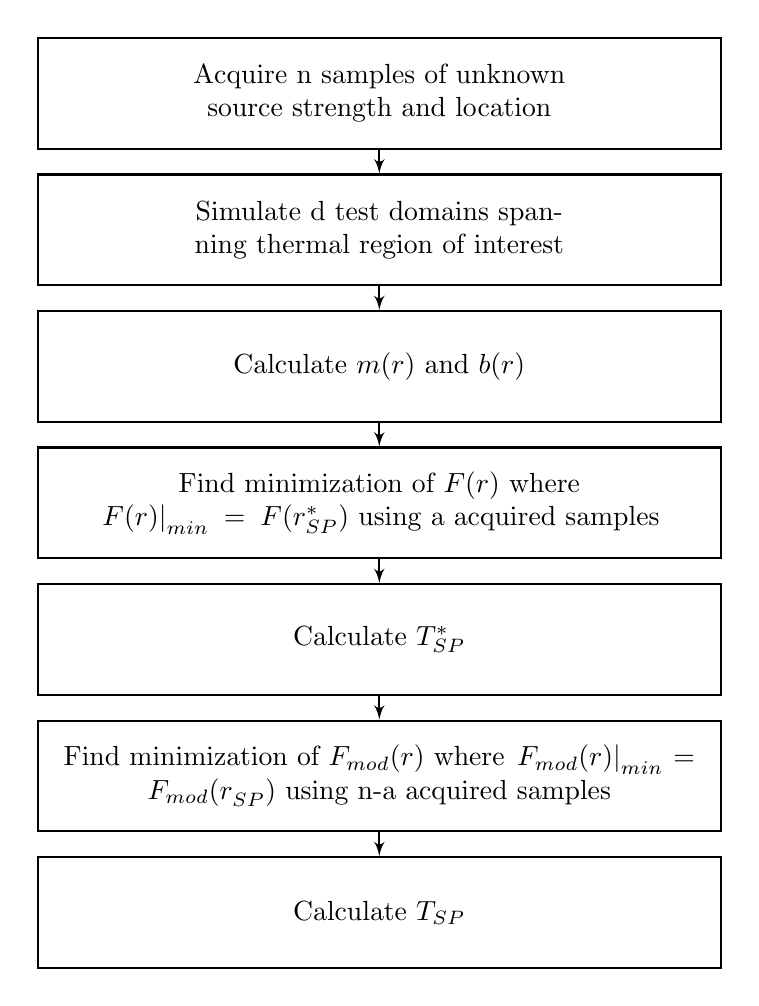
\begin{tikzpicture}[auto,
    %decision/.style={diamond, draw=black, thick, fill=white,
    %text width=8em, text badly centered,
    %inner sep=1pt, font=\sffamily\small},
    block_center/.style ={rectangle, draw=black, thick, fill=white,
      text width=24em, text centered,
      minimum height=4em},
    block_left/.style ={rectangle, draw=black, thick, fill=white,
      text width=16em, text ragged, minimum height=4em, inner sep=6pt},
    block_noborder/.style ={rectangle, draw=none, thick, fill=none,
      text width=18em, text centered, minimum height=1em},
    block_assign/.style ={rectangle, draw=black, thick, fill=white,
      text width=18em, text ragged, minimum height=3em, inner sep=6pt},
    block_lost/.style ={rectangle, draw=black, thick, fill=white,
      text width=16em, text ragged, minimum height=3em, inner sep=6pt},
      line/.style ={draw, thick, -latex', shorten >=0pt}]
    % outlining the flowchart using the PGF/TikZ matrix funtion
    \matrix [column sep=5mm,row sep=3mm] {
			\node [block_center] (acquire) {Acquire n samples of unknown source strength and location};\\
		  \node [block_center] (sim) {Simulate d test domains spanning thermal region of interest};	\\		
			\node [block_center] (calcm) {Calculate $m( \bv r)$ and $b( \bv r)$};	\\		
			\node [block_center] (minf) {Find minimization of $F( \bv r)$ where $\left. F( \bv r) \right|_{min} = F(\bv{r^{\ast}_{SP}})$ using a acquired samples};	\\					
			\node [block_center] (calcts) {Calculate $T^{\ast}_{SP}$};	\\		
			\node [block_center] (minfmod) {Find minimization of $F_{mod}(\bv r)$ where $\left. F_{mod}( \bv r) \right|_{min} = F_{mod}(\bv{r^{ }_{SP}})$ using n-a acquired samples};	\\					
			\node [block_center] (calct) {Calculate $T_{SP}$};	\\					
   };% end matrix
    % connecting nodes with paths
    \begin{scope}[every path/.style=line]
      \path (acquire)     -- (sim);
			\path (sim)     -- (calcm);
			\path (calcm)     -- (minf);
			\path (minf)     -- (calcts);
			\path (calcts)     -- (minfmod);
			\path (minfmod)     -- (calct);			
    \end{scope}		
  \end{tikzpicture}
\caption{Flowchart of the presented methodology}
\label{fig:flowchart}
\end{figure}




\section{Results and discussions}

To separate experimental error from algorithm error, the method will initially only be applied to simulation results.  To further define how and where the error in predictions occur, a systematic set of test cases was performed.  Starting with the simplest case, where both horizontal source location $x_S$ and vertical source location $y_S$ are known a priori, and finishing with the most difficult, where none of the horizontal source location $x_S$, the vertical source location $y_S$, and the source temperature $T_S$ are known a priori.  It is worth noting only a small subset of performed numerical simulations and experimental results are presented in this study.

In the first test case, the predictor - corrector method is applied to the problem where both $x_S$ and $y_S$ are known.  Upon examining \cref{eq:linearset} or \cref{eq:linearset2} with fixed $x_S$ and $y_S$, it becomes obvious that, knowing the temperature at one location, results in a simplification of the predictor - corrector method to the exact solution of the inverse problem.  An example of a few test cases are shown in \cref{tab:typeA}.  The prediction error of source temperature of this inverse calculation is negligible for all cases within the plume.  This error is likely caused by neglecting variations in density and buoyancy, however this was not verified.  Alternative forms of error such as radiation were not yet considered due to the data sets compared are simulation results only.

The following, \cref{tab:typeA,tab:typeB,tab:typeC,tab:typeD,tab:typeE},  are similar and may be read as such.  Each column consists of a specified free stream velocity $U_{\infty}$ and a specified source temperature $T_S$.  Again, source temperature may be replaced with source heat flux.  Each row is labeled by a data sampling datum location ($x_S$, $y_S$), in millimeters.  As explained previously, the predictor phase uses three points arranged horizontally at and behind the datum location with $1.0\,mm$ spacing, and the corrector phase uses three points arranged vertically at and above the datum location with $1.0\,mm$ spacing.

\Cref{eq:error} is the means by which the error is calculated.  The constant parameters for the simulation tests are listed 

\begin{subequations}
\begin{align}
error_{temp} (\%) &= \frac{\left|T_{SP}-T_S\right| }{T_S-T_{\infty}} \times 100 \\
error_{x-location} (\%) &= \frac{\left|x_{SP}-x_S\right|}{x_S} \times 100 \\
error_{y-location} (\%) &= \frac{\left|y_{SP}-y_S\right|}{y_S} \times 100 
\end{align}
\label{eq:error}
\end{subequations}

\begin{table}[!h!t!b!p]
\begin{center}
\begin{tabular}{ l | c c c c}
 $U_{\infty}$ $(m/s)$ & 0.6 & 0.6 & 1.0 & 1.0 \\ \hline
 $T_S$ $(K)$ & 375 & 425 & 375 & 425  \\ \hline \hline
 Location (x,y) & \\
 40 mm, 1 mm & $0.01\%$ & $0.01\%$ & $0.01\%$ & $0.02\%$ \\ \hline
 40 mm, 2 mm & $0.02\%$ & $0.01\%$ & $0.11\%$ & $0.19\%$ \\ \hline
 60 mm, 1 mm & $0.01\%$ & $0.01\%$ & $0.00\%$ & $0.00\%$ \\ \hline
 60 mm, 2 mm & $0.02\%$ & $0.02\%$ & $0.01\%$ & $0.03\%$ \\ \hline
 80 mm, 1 mm & $0.01\%$ & $0.01\%$ & $0.01\%$ & $0.01\%$ \\ \hline
 80 mm, 2 mm & $0.01\%$ & $0.01\%$ & $0.04\%$ & $0.07\%$ \\ \hline
 \end{tabular}
\caption{Error in the prediction of $T_S$ from several sampled cases within the plume with $x_S$ and $y_S$ known}
\label{tab:typeA}
\end{center}
\end{table}

The next type of problem has both the plume source strength and the elevation known.  That is to say both $T_S$ and $y_S$ are known a priori.  With the source strength known, the predictor - corrector method simplifies to just the corrector half of the method.  The prediction error of the $x_S$ location is small (shown in \cref{tab:typeB}), but not insignificant.  The error for this case is less than $1.0\%$ when testing within the plume.  This error is caused by again neglecting the variations in density and buoyancy, but also the random errors introduced by the genetic algorithm during the minimization process.

\begin{table}[!h!t!b!p]
\begin{center}
\begin{tabular}{ l | c c c c}
 $U_{\infty}$ $(m/s)$ & 0.6 & 0.6 & 1.0 & 1.0 \\ \hline
 $T_S$ $(K)$ & 375 & 425 & 375 & 425  \\ \hline \hline
 Location (x,y) & \\
 40 mm, 1 mm & $0.50\%$ & $0.28\%$ & $0.29\%$ & $0.01\%$ \\ \hline
 40 mm, 2 mm & $0.33\%$ & $0.31\%$ & $0.63\%$ & $0.09\%$ \\ \hline
 60 mm, 1 mm & $0.53\%$ & $0.29\%$ & $0.36\%$ & $0.08\%$ \\ \hline
 60 mm, 2 mm & $0.87\%$ & $0.47\%$ & $0.72\%$ & $0.23\%$ \\ \hline
 80 mm, 1 mm & $0.22\%$ & $0.13\%$ & $0.06\%$ & $0.03\%$ \\ \hline
 80 mm, 2 mm & $0.60\%$ & $0.40\%$ & $0.48\%$ & $0.11\%$ \\ \hline
 \end{tabular}
\caption{Error in the prediction of the horizontal location $x_S$ from several sampled cases within the plume with source temperature $T_S$ and $y_S$ known}
\label{tab:typeB}
\end{center}
\end{table}


The case where $T_S$ is known is very similar to the previous case, and also reduces to the corrector half.  The error here is identical to the previous case, that is the errors introduced by neglecting the variations in density and buoyancy, and random errors introduced by the genetic algorithm.  As one might expect the $x_S$ error for this case is similar to the previous one.  The $y_S$ error is larger, as expected.  The $y$ direction error calculation is more sensitive than that in the $x$ direction, as the values are numerically smaller.  Thus equivalent magnitude errors between $x_S$ and $y_S$ directions cause a more significant relative error in $y_S$.  The error of predicted $x_S$ and $y_S$ may be found in \cref{tab:typeC}.

\begin{table}[!h!t!b!p]
\begin{center}
\begin{tabular}{ l | l c c c c}
 $U_{\infty}$ $(m/s)$ & & 0.6 & 0.6 & 1.0 & 1.0 \\ \hline
 $T_S$ $(K)$ & & 375 & 425 & 375 & 425  \\ \hline \hline
 Location (x,y) & \\
 40 mm, 1 mm & X & $0.16\%$ & $0.06\%$ & $0.31\%$ & $0.08\%$ \\
 						 & Y & $5.53\%$ & $2.82\%$ & $2.72\%$ & $0.48\%$ \\ \hline
 40 mm, 2 mm & X & $0.26\%$ & $0.26\%$ & $0.14\%$ & $0.06\%$ \\ 
 						 & Y & $1.84\%$ & $0.67\%$ & $1.03\%$ & $0.08\%$ \\ \hline
 60 mm, 1 mm & X & $0.19\%$ & $0.15\%$ & $0.03\%$ & $0.09\%$ \\ 
						 & Y & $3.61\%$ & $1.62\%$ & $1.77\%$ & $0.08\%$ \\ \hline
 60 mm, 2 mm & X & $0.07\%$ & $0.01\%$ & $0.57\%$ & $0.57\%$ \\ 
   					 & Y & $2.39\%$ & $1.67\%$ & $2.02\%$ & $1.34\%$ \\ \hline
 80 mm, 1 mm & X & $0.00\%$ & $0.01\%$ & $0.12\%$ & $0.08\%$ \\ 
  					 & Y & $3.47\%$ & $1.85\%$ & $1.43\%$ & $0.33\%$ \\ \hline
 80 mm, 2 mm & X & $0.18\%$ & $0.18\%$ & $0.84\%$ & $0.82\%$ \\ 
 						 & Y & $2.37\%$ & $1.68\%$ & $2.35\%$ & $1.89\%$ \\ \hline
 \end{tabular}
\caption{Error in predicting $x_S$, $y_S$ from several sampled cases within the plume with $T_S$ known}
\label{tab:typeC}
\end{center}
\end{table}


The last case is where none of the $x_S$, $y_S$, and $T_S$ information is known a priori.  The error in this case is compounded between the three parameters.  Small errors in predicted source strength may yield large errors in location and vice-versa.  The results of $x_S$ and $y_S$ are similar to that found from the previous case, and results are shown in \cref{tab:typeD}.  The error in prediction of the source temperature is under $1.5\%$ in all sampled cases.

\begin{table}[!h!t!b!p]
\begin{center}
\begin{tabular}{ l | l c c c c}
 $U_{\infty}$ $(m/s)$ & & 0.6 & 0.6 & 1.0 & 1.0 \\ \hline
 $T_S$ $(K)$ & & 375 & 425 & 375 & 425  \\ \hline \hline
 Location (x,y) & \\
 40 mm, 1 mm & X & $0.28\%$ & $0.28\%$ & $0.37\%$ & $0.10\%$ \\
 						 & Y & $4.86\%$ & $4.86\%$ & $2.37\%$ & $0.42\%$ \\
 						 & T & $0.68\%$ & $0.78\%$ & $0.52\%$ & $0.07\%$ \\ \hline
 40 mm, 2 mm & X & $0.11\%$ & $0.11\%$ & $0.24\%$ & $0.04\%$ \\ 
 						 & Y & $1.06\%$ & $1.06\%$ & $0.77\%$ & $0.31\%$ \\ 
 						 & T & $1.08\%$ & $1.08\%$ & $0.85\%$ & $0.07\%$ \\ \hline
 60 mm, 1 mm & X & $0.01\%$ & $0.01\%$ & $0.09\%$ & $0.04\%$ \\ 
						 & Y & $3.93\%$ & $3.93\%$ & $1.69\%$ & $0.06\%$ \\ 
						 & T & $0.32\%$ & $0.32\%$ & $0.21\%$ & $0.05\%$ \\ \hline
 60 mm, 2 mm & X & $0.27\%$ & $0.27\%$ & $0.74\%$ & $0.59\%$ \\ 
   					 & Y & $2.26\%$ & $2.26\%$ & $1.89\%$ & $1.29\%$ \\ 
   					 & T & $0.67\%$ & $0.77\%$ & $0.69\%$ & $0.25\%$ \\ \hline
 80 mm, 1 mm & X & $0.07\%$ & $0.07\%$ & $0.12\%$ & $0.07\%$ \\ 
  					 & Y & $2.89\%$ & $2.89\%$ & $1.38\%$ & $0.35\%$ \\ 
  					 & T & $0.25\%$ & $0.25\%$ & $0.12\%$ & $0.00\%$ \\ \hline
 80 mm, 2 mm & X & $0.36\%$ & $0.36\%$ & $0.86\%$ & $0.73\%$ \\ 
 						 & Y & $2.19\%$ & $2.19\%$ & $2.34\%$ & $1.93\%$ \\ 
 						 & T & $0.46\%$ & $0.46\%$ & $0.33\%$ & $0.13\%$ \\ \hline
 \end{tabular}
\caption{Error in predicting $x_S$, $y_S$, $T_S$ from several sample cases within the plume}
\label{tab:typeD}
\end{center}
\end{table}

\begin{table}[!h!t!b!p]
\begin{center}
\begin{tabular}{ l c}
\hline
Parameter & Value \\ \hline
$T_{\infty}\, (K)$ & $293$ \\
$P_{\infty}\, (kPa)$ & $101.32$ \\
$T_{SA},\, T_{SB}\, (K)$ & $350,\,450$ \\
n stage 1 & 3 \\
n stage 2 & 3 \\
$\delta x,\, \delta y $ stage 1 & $1.0\,mm,\,0.0\,mm$ \\
$\delta x,\, \delta y $ stage 2 & $0.0\,mm,\,1.0\,mm$ \\ \hline
 \end{tabular}
 \end{center}
\caption{Test parameters for the simulations}
\label{tab:simparam}
\end{table}


\subsection{Experimental Results}

An evaluation of the methodology against experimental data was performed, and the results are shown in \cref{tab:typeE}.  At first glance, the methodology does not appear to fare well with respsect to error, as compared to that for the simulation results.  The issue is the use of relative error versus absolute error.  In the numerical simulation tests use of relative error made the results clear.  In the case of the experiment, both absolute error and relative error give a misrepesentation of the results due to the large length scale in x compared to y.

The X-direction error for $x=40\, mm$ and $x=60\, mm$ never goes above $6.7\% $.  This is a reasonable expected error for the X-direction.  The Y-direction error for $x=40\, mm$ and $x=60\, mm$ never goes above $10\% $.  This seems a little high until you look at the absolute value of that error of $0.2\, mm$.  This error no longer seems to be a particularly large value when considering the lengths involved with the other direction.  The temperature error for $x=40\, mm$ and $x=60\, mm$, does not go above $5\% $ error.  This is very reasonable for the temperature prediction.

The problem arises when one starts looking at the errors for $x=80\, mm$.  The errors are very high.  This high error can easily be explained, looking back at \cref{fig:mVSxy,fig:bVSxy}.  In both cases, the curves asymptotically tend towards a single value, meaning the methodology will not be able to differentiate values far downstream.  This compounds with the natural experimental error, resulting in a finite distance down stream that this methodology is effective.  This distance is a function of both $U_{\infty}$ and $T_S$.  This makes sense from a turbulence stand point, since one would expect the flow field to eventually lead to uniform temperature.  As discussed previously $\frac{\partial m}{\partial x}$ and $\frac{\partial b}{\partial x}$ need to be large with respect to the magnitude of the error for the result to be essentially unique.  If the temperature is uniform then this is not the case and no unique solution can be found.

Some of the errors in this case must be from the simulation errors.  That is to say the simulations do not $100\%$ match the physical experimental data.  Some of the discrepancies may be explained by not simulating radiation, the inherent errors in the turbulence model, and difficulties simulating the transitional turbulence regime.

\begin{table}[!h!t!b!p]
\begin{center}
\begin{tabular}{ l | l c c c c}
 $U_{\infty}$ $(m/s)$ & & 0.6 & 0.6 & 1.0 & 1.0 \\ \hline
 $T_S$ $(K)$ & & 375 & 425 & 375 & 425  \\ \hline \hline
 Location (x,y) & \\
 40 mm, 1 mm & X & $0.0\%$ & $2.5\%$ & $5.0\%$ & $0.0\%$ \\
 						 & Y & $0.0\%$ & $10.\%$ & $2.0\%$ & $10.\%$ \\
 						 & T & $1.2\%$ & $1.8\%$ & $0.0\%$ & $1.1\%$ \\ \hline
 40 mm, 2 mm & X & $2.5\%$ & $2.5\%$ & $2.5\%$ & $2.5\%$ \\ 
 						 & Y & $10.\%$ & $10.\%$ & $10.\%$ & $5.0\%$ \\ 
 						 & T & $1.7\%$ & $2.0\%$ & $0.7\%$ & $1.9\%$ \\ \hline
 60 mm, 1 mm & X & $0.0\%$ & $3.3\%$ & $6.7\%$ & $0.0\%$ \\ 
						 & Y & $0.0\%$ & $8.0\%$ & $5.0\%$ & $2.0\%$ \\ 
						 & T & $1.1\%$ & $4.2\%$ & $3.3\%$ & $4.9\%$ \\ \hline
 60 mm, 2 mm & X & $6.7\%$ & $6.7\%$ & $3.7\%$ & $3.3\%$ \\ 
   					 & Y & $10.\%$ & $10.\%$ & $10.\%$ & $10.\%$ \\ 
   					 & T & $1.5\%$ & $4.9\%$ & $3.2\%$ & $3.2\%$ \\ \hline
 80 mm, 1 mm & X & $0.0\%$ & $7.5\%$ & $3.7\%$ & $0.0\%$ \\ 
  					 & Y & $1.0\%$ & $40.\%$ & $10.\%$ & $10.\%$ \\ 
  					 & T & $6.1\%$ & $38.\%$ & $54.\%$ & $32.\%$ \\ \hline
 80 mm, 2 mm & X & $5.0\%$ & $12.\%$ & $2.5\%$ & $1.2\%$ \\ 
 						 & Y & $25.\%$ & $35.\%$ & $10.\%$ & $5.0\%$ \\ 
 						 & T & $8.8\%$ & $29.\%$ & $41.\%$ & $54.\%$ \\ \hline
 \end{tabular}
\caption{Error in predicting $x_S$, $y_S$, $T_S$ from several sample cases within the plume}
\label{tab:typeE}
\end{center}
\end{table}


\section{Conclusions}

A predictor - corrector approach for solving inverse convection problems was developed and tested against both numerical and experimental results.  The method was developed starting with the previous work \cite{knight,rossmann} and employing sensitivity analysis of the problem.  

The results from all of the simulation tests show a relative source strength prediction error of less than $1\%$ in all cases tested within the plume.  The relative source location prediction error was less than $1\%$ for the free stream direction and less than $6\%$ for the direction perpendicular to the free stream.  Experimental tests indicate that the algorithm is only slightly less accurate, with the error increasing to $5\%$, for prediction of the source strength, and $5\%$ for prediction of the free stream coordinate location of the source.  The coordinate perpendicular to the free stream has an error of $10\%$.  While the $10\%$ seems significant the result in physical terms is only $0.2 \, mm$.

The predictor-corrector method lends itself to further investigations.  One major focus is the size and shape of the sampling patterns used.  Optimization of the sampling pattern would reduce the error associated with the method while keeping the number of samples to an absolute minimum.  Another focus is a full error analysis of the parameters.  The goal would be to develop a domain of error, a function to determine for what parameter values the methodology is within acceptable error.

The methodology could be useful in similar experimental cases, such as a jet in a crosswind or a plume with  crosswind.  If the methodology could be furthered to a more mature state (e.g. transient and three dimensional validation), it could be applicable in any number of inverse convection problems.  Examples of applications include fires in enclosures and/or urban environments\cite{hu}	, such as tunnels\cite{blanchard}, rooms, and buildings.

\appendix

\bibliography{Bibliography}{}
\bibliographystyle{model1-num-names}
\end{document}